\documentclass[
	% -- opções da classe memoir --
	12pt,				% tamanho da fonte
	openright,			% capítulos começam em pág ímpar (insere página vazia caso preciso)
	oneside,			% para impressão em verso e anverso. Oposto a oneside
	a4paper,
	left=1cm,
	right=4cm,
	top=3cm,
	bottom=8cm,			% tamanho do papel. 
	% -- opções da classe abntex2 --
	%chapter=TITLE,		% títulos de capítulos convertidos em letras maiúsculas
	%section=TITLE,		% títulos de seções convertidos em letras maiúsculas
	%subsection=TITLE,	% títulos de subseções convertidos em letras maiúsculas
	%subsubsection=TITLE,% títulos de subsubseções convertidos em letras maiúsculas
	% -- opções do pacote babel --
	english,			% idioma adicional para hifenização
	french,				% idioma adicional para 
	hifenização
	spanish,			% idioma adicional para hifenização
	brazil				% o último idioma é o principal do documento
	]{abntex2}


% --- 
% CONFIGURAÇÕES DE PACOTES
% --- 
% ---
% Pacotes básicos 
% ---



\renewcommand{\baselinestretch}{1.5}
\usepackage{helvet}
\renewcommand{\familydefault}{\sfdefault}			% Usa a fonte arial Modern			
\usepackage[T1]{fontenc}		% Selecao de codigos de fonte.
\usepackage[utf8]{inputenc}		% Codificacao do documento (conversão automática dos acentos)
\usepackage{lastpage}			% Usado pela Ficha catalográfica
\usepackage{indentfirst}		% Indenta o primeiro parágrafo de cada seção.
\usepackage{color}				% Controle das cores
\usepackage{graphicx}			% Inclusão de gráficos
\usepackage{microtype} 			% para melhorias de justificaçã

\usepackage{ufc-abntex2}




		
% ---
% Pacotes adicionais, usados apenas no âmbito do Modelo Canônico do abnteX2
% ---
\usepackage{lipsum}				% para geração de dummy text
% ---

% ---
% Pacotes de citações
% ---
\usepackage[brazilian,hyperpageref]{backref}	 % Paginas com as citações na bibl
\usepackage[alf]{abntex2cite}	% Citações padrão ABNT

% ---
% Configurações do pacote backref
% Usado sem a opção hyperpageref de backref
%\renewcommand{\backrefpagesname}{Citado na(s) página(s):~}
% Texto padrão antes do número das páginas
%\renewcommand{\backref}{}
% Define os textos da citação
\renewcommand*{\backrefalt}[4]{
	}%\\renewcommand{\normalrulethickness}{0pt}
\makeheadrule{abntheadings}{\textwidth}{0pt}

% ---

% ---
% Configurações de aparência do PDF final

% alterando o aspecto da cor azul
\definecolor{blue}{RGB}{41,5,195}

% informações do PDF
\makeatletter
\hypersetup{
     	%pagebackref=true,
		pdftitle={\@title}, 
		pdfauthor={\@author},
    	pdfsubject={\imprimirpreambulo},
	    pdfcreator={LaTeX with abnTeX2},
		pdfkeywords={abnt}{latex}{abntex}{abntex2}{trabalho acadêmico}, 
		colorlinks=true,       		% false: boxed links; true: colored links
    	linkcolor=black,          	% color of internal links
    	citecolor=black,        		% color of links to bibliography
    	filecolor=magenta,      		% color of file links
		urlcolor=black,
		bookmarksdepth=4
}
\makeatother
% --- 

% --- 
% Espaçamentos entre linhas e parágrafos 
% --- 

% O tamanho do parágrafo é dado por:
\setlength{\parindent}{1.3cm}

% Controle do espaçamento entre um parágrafo e outro:
\setlength{\parskip}{0.2cm}  % tente também \onelineskip

% ---
% compila o indice
% ---
\makeindex
% ---

\setlrmarginsandblock{3cm}{2cm}{*}
\setulmarginsandblock{3cm}{2cm}{*}
\checkandfixthelayout
\pagestyle{myheadings}

\usepackage{float}
%\usepackage[a4paper,bottom=2cm,top=3cm,left=3cm,right=2cm]{geometry}
\usepackage{acronym}
\usepackage{listings}
\usepackage{xcolor}
\usepackage{subcaption}
\usepackage{anyfontsize}

\usepackage{caption}
\DeclareCaptionFont{xxviii}{\fontsize{11}{11}\selectfont}
\captionsetup{font=xxviii}
\lstset{ %
	texcl=true,
	aboveskip=5pt,
	belowskip=5pt,
	backgroundcolor=\color{cyan},   % choose the background color; you must add \usepackage{color} or \usepackage{xcolor}; should come as last argument
	basicstyle=\footnotesize,        % the size of the fonts that are used for the code
	breakatwhitespace=false,         % sets if automatic breaks should only happen at whitespace
	breaklines=true,                 % sets automatic line breaking
	captionpos=t,                    % sets the caption-position to bottom
	%	commentstyle=\color{mygreen},    % comment style
	deletekeywords={...},            % if you want to delete keywords from the given language
	escapeinside={\%*}{*)},          % if you want to add LaTeX within your code
	extendedchars=true,              % lets you use non-ASCII characters; for 8-bits encodings only, does not work with UTF-8
	frame=single,	                   % adds a frame around the code
	keepspaces=true,                 % keeps spaces in text, useful for keeping indentation of code (possibly needs columns=flexible)
	keywordstyle=\color{blue},       % keyword style
	language=bash,                 % the language of the code
	morekeywords={*,...},            % if you want to add more keywords to the set
	numbers=none,                    % where to put the line-numbers; possible values are (none, left, right)
	numbersep=5pt,                   % how far the line-numbers are from the code
	%	numberstyle=\tiny\color{mygray}, % the style that is used for the line-numbers
	rulecolor=\color{green},         % if not set, the frame-color may be changed on line-breaks within not-black text (e.g. comments (green here))
	showspaces=false,                % show spaces everywhere adding particular underscores; it overrides 'showstringspaces'
	showstringspaces=false,          % underline spaces within strings only
	showtabs=false,                  % show tabs within strings adding particular underscores
	stepnumber=2,                    % the step between two line-numbers. If it's 1, each line will be numbered
	%	stringstyle=\color{mymauve},     % string literal style
	tabsize=2,	                   % sets default tabsize to 2 spaces
	title=\lstname                   % show the filename of files included with \lstinputlisting; also try caption instead of title
}

\lstset{%
	basicstyle=\small\ttfamily,language={bash},   numbersep=5mm, numbers=left, numberstyle=\tiny, % number style
	breaklines=true,frame=single,framexleftmargin=8mm, xleftmargin=	8mm,
	prebreak = \raisebox{0ex}[0ex][0ex]{\ensuremath{\hookleftarrow}},
	backgroundcolor=\color{green!6},frameround=fttt,escapeinside=??,
	rulecolor=\color{red},
	morekeywords={% Give key words here                                         % keywords
		maketitle},
	keywordstyle=\color[rgb]{0,0,1},                    % keywords
	commentstyle=\color[rgb]{0.133,0.545,0.133},    % comments
	stringstyle=\color[rgb]{0.627,0.126,0.941}  % strings
	%columns=fullflexible   
}%
\renewcommand{\lstlistingname}{Quadro}
\renewcommand\lstlistlistingname{Lista De Quadros}
\usepackage{titlesec}

\usepackage{chngcntr}
\AtBeginDocument{\counterwithout{lstlisting}{chapter}}

\titleformat{\section}    
{\normalfont\fontfamily{phv}\fontsize{14}{17}\bfseries}{\thesection}{1em}{}

\titleformat{\subsection}    
{\normalfont\fontfamily{phv}\fontsize{14}{17}\bfseries}{\thesubsection}{1em}{}

%%%%%%%%%%%%%%%%%%%%%%%%%%%%%%%%%%%%%%%%%%%%%%%%%%%%%%%%%%%
\newcommand{\chapfnt}{\fontsize{16}{22}}




%%%%%%%%%%%%%%%%%%%%%%%%%%%%%%%%%%%%%%%%%%%%%%%%%%%%%%%%%%%
%FORMATAR SOMENTE CABEÇALHOS DAS SEÇÕES
%\titleformat{\chapter}    
%{\normalfont\fontfamily{phv}\fontsize{16}{10}\bfseries}{\thechapter}{1em}{}


% Informações de dados para CAPA e FOLHA DE ROSTO
\titulo{\uppercase{Desenvolvimento de Progressives Web Apps e Análise Comparativa com Aplicações Móveis Nativas}}
\autor{Pedro Cruz}
\local{Fortaleza, Ceará}
\data{2019}
\orientador{Prof Msc. Fred Viana}


\instituicao{%
FACULDADE LOURENÇO FILHO

\par
BACHARELADO EM SISTEMAS  DE  INFORMAÇÃO 
}
%\tipotrabalho{Trabalho de Conclusão de Curso (Monografia)}
%\preambulo{Trabalho de Conclusão de Curso submetido à Coordenação do Curso de Engenharia de Software do Campus Quixadá da Universidade Federal do Ceará, como requisito parcial para obtenção do Título de Bacharel em Engenharia de Software.}


\begin{document}
\frenchspacing 

% ----------------------------------------------------------
% ELEMENTOS PRÉ-TEXTUAIS
% ----------------------------------------------------------
\pretextual
% Capa
\imprimircapa
% Folha de rosto (* indica que haverá a ficha bibliográfica)
\imprimirfolhaderosto*

% Ficha Bibliográfica
%% ---
% Inserir a ficha bibliografica
% ---

% Isto é um exemplo de Ficha Catalográfica, ou ``Dados internacionais de
% catalogação-na-publicação''. Você pode utilizar este modelo como referência. 
% Porém, provavelmente a biblioteca da sua universidade lhe fornecerá um PDF
% com a ficha catalográfica definitiva após a defesa do trabalho. Quando estiver
% com o documento, salve-o como PDF no diretório do seu projeto e substitua todo
% o conteúdo de implementação deste arquivo pelo comando abaixo:
%
% \begin{fichacatalografica}
%     \includepdf{fig_ficha_catalografica.pdf}
% \end{fichacatalografica}
\begin{fichacatalografica}
	\vspace*{\fill}					% Posição vertical
	\hrule							% Linha horizontal
	\begin{center}					% Minipage Centralizado
	\begin{minipage}[c]{12.5cm}		% Largura
	
%	\imprimirautor
	Cabral,Guylherme Tabosa
	
	\hspace{0.5cm} \imprimirtitulo  / \imprimirautor. --
	\imprimirlocal, \imprimirdata-
	
	\hspace{0.5cm} \pageref{LastPage} p. : il. (algumas color.) ; 30 cm.\\
	
	\hspace{0.5cm} \imprimirorientadorRotulo~\imprimirorientador\\
	
	\hspace{0.5cm}
	\parbox[t]{\textwidth}{\imprimirtipotrabalho~--~\imprimirinstituicao,\imprimirlocal,
	\imprimirdata.}\\
	
	\hspace{0.5cm}
		1. Gerência de Configuração.
		2. Integração Contínua.
		3. Processo de Software.
		4. Qualidade de Software
		I. Almeida, Carlos Diego Andrade de.
		II. Universidade Federal do Ceará.
		III. \MakeLowercase{{\imprimirtitulo}}.\\ 			
	
	\hspace{8.75cm} CDU 02:141:005.7\\
	
	\end{minipage}
	\end{center}
	\hrule
\end{fichacatalografica}
% ---

% Errata
%% ---
% Inserir errata
% ---
\begin{errata}
Elemento opcional da NORMA. Exemplo:

\vspace{\onelineskip}

FERRIGNO, C. R. A. \textbf{Tratamento de neoplasias ósseas apendiculares com
reimplantação de enxerto ósseo autólogo autoclavado associado ao plasma
rico em plaquetas}: estudo crítico na cirurgia de preservação de membro em
cães. 2011. 128 f. Tese (Livre-Docência) - Faculdade de Medicina Veterinária e
Zootecnia, Universidade de São Paulo, São Paulo, 2011.

\begin{table}[htb]
\center
\footnotesize
\begin{tabular}{|p{1.4cm}|p{1cm}|p{3cm}|p{3cm}|}
  \hline
   \textbf{Folha} & \textbf{Linha}  & \textbf{Onde se lê}  & \textbf{Leia-se}  \\
    \hline
    1 & 10 & auto-conclavo & autoconclavo\\
   \hline
\end{tabular}
\end{table}

\end{errata}
% ---


% Folha de Aprovação
%% ---
% Inserir folha de aprovação
% ---

% Isto é um exemplo de Folha de aprovação, elemento obrigatório da NBR
% 14724/2011 (seção 4.2.1.3). Você pode utilizar este modelo até a aprovação
% do trabalho. Após isso, substitua todo o conteúdo deste arquivo por uma
% imagem da página assinada pela banca com o comando abaixo:
%
% \includepdf{folhadeaprovacao_final.pdf}
%
\begin{folhadeaprovacao}

  \begin{center}
    {\ABNTEXchapterfont\bfseries\Large\imprimirautor}
    \vspace{1cm}

    \begin{center}
      \ABNTEXchapterfont\bfseries\Large\imprimirtitulo
    \end{center}

    \vspace{2cm}
    \begin{minipage}{\textwidth}
        \imprimirpreambulo
        \\ \\
        Área de concentração: Computação
        \\ \\ \\
        Aprovada em: 19 / novembro/ 2014
    \end{minipage}%
     
    \vspace{2cm}
	\textbf{BANCA EXAMINADORA}
   \end{center}
	

   \assinatura{\imprimirorientador \space (Orientador) \\ Universidade Federal do Ceará (UFC)}
 
	\assinatura{Prof Msc. Camilo Camilo Almendra \space (Membro) \\ Universidade Federal do Ceará (UFC)}
   
   \assinatura{Prof Msc. Régis Pires Magalhães \space (Membro) \\ Universidade Federal do Ceará (UFC)}
   %\assinatura{\textbf{Professor} \\ Convidado 2}
   %\assinatura{\textbf{Professor} \\ Convidado 3}
      
%   \begin{center}
%    \vspace*{0.5cm}
%    {\large\imprimirlocal}
%    \par
%    {\large\imprimirdata}
%    \vspace*{1cm}
%  \end{center}
  
\end{folhadeaprovacao}
% ---

%\imprimirfolhadeaprovacao

% Dedicatória
%% ---
% Dedicatória
% ---
\begin{dedicatoria}
   \vspace*{\fill}
   	\begin{flushright}
   \noindent
   A minha família principalmente meus avós, minha mãe, meu irmão, meu pai e a Mikaely.
   	\end{flushright}
\end{dedicatoria}
% ---

% Agradecimentos
%% ---
% Agradecimentos
% ---
\begin{agradecimentos}
	 Agradeço primeiramente a Deus por me dar sabedoria, vontade e disposição para concluir este trabalho, sem ele nada seria possível.
	 
	 A minha mãe Rejane, pelo exemplo de mulher e amor. Por sempre cuidar de mim mesmo quando não estive perto por todos esses anos de universidade.
	 
	 A meu avô Nonato, pelo símbolo de pai, modelo de ser humano e seu meu maior exemplo de vida.
	 
	 A minha avó Rita, por todo o amor, força e cuidado, minha segunda mãe.
	 
	 A meu irmão Felype por sempre partilhar comigo momentos bons e ruins e cuidar de mim quando precisei.
	 
	 A meu pai João por ensinar que o trabalho sempre gera resultados, e que o esforço é seu maior aliado para o sucesso. 
	 
	 A minha família pela ajuda e cuidado.
	 
	 A Mikaely por ter me aturado nos momentos de confusão, medo, raiva, angústia e outros mais, sua presença ao meu lado me fez mais forte e focado nos objetivos.
	 
	 A meus amigos de faculdade, por todos esses anos de companheirismo, felicidades e ajudas.
	 
	 A meu orientador Carlos Diego por me guiar na obtenção do melhor resultado possível e disponibilidade e interesse neste projeto.
	 
	 A UFC e seus funcionários por fornecer as ferramentas para que pudesse evoluir meus conhecimentos. Obrigado a todos.
\end{agradecimentos}
% ---

% Epígrafe
%% ---
% Epígrafe
% ---
\begin{epigrafe}
    \vspace*{\fill}
	\begin{flushright}
		\textit{``Observo a mim mesmo em silêncio, \\
		porque é nele onde mais e melhor se diz, \\
		Me  ensino a ser mais tolerante, não julgar ninguém \\
		E com isso ser mais feliz.\\
		''}
	\end{flushright}
\end{epigrafe}
% ---

% RESUMOS
%% resumo em português
\setlength{\absparsep}{18pt} % ajusta o espaçamento dos parágrafos do resumo
\begin{resumo}
 
O desenvolvimento ágil está cada dia mais presente no cotidiano das empresas desenvolvedoras de software. A crescente busca por agilidade no desenvolvimento e a competitividade do mercado impactam na existência deste cenário. Portanto, muitas empresas buscam aplicar as metodologias definidas neste ramo de desenvolvimento em seu processos, porém, essa não é uma tarefa simples. A definição e implantação dessas práticas realizadas de maneira não suficientemente adequada podem trazer resultados adversos ao esperado. Portanto este trabalho teve como objetivo implantar a utilização de uma ferramenta de integração contínua em uma fábrica de software, o Núcleo de Práticas em Informática (NPI) da UFC - Campus Quixadá. Uma ferramenta de integração contínua está inserida em uma das práticas definidas pelo Extreme Programming (XP). Para a realização deste objetivo fora analisado o processo vigente executado no NPI, além da experiência do autor que era um membro desta fábrica de software. Somado a esta etapa foi definida a ferramenta de integração contínua a ser implantada de acordo com um conjunto de característica especificadas, o conhecimento dos membros da fábrica acerca de Gerência de configuração e Integração Contínua foi avaliado, e por fim, a implantação, com a definição de pontos positivos e negativos encontrados na implantação.


 \textbf{Palavras-chaves}: Integração Contínua. Desenvolvimento Ágil. Gerenciamento de Configuração.
\end{resumo}
%% resumo em inglês
\begin{resumo}[Abstract]
 \begin{otherlanguage*}{english}
The agile development is day by day inserted on the quotidian of software development companies. The growing seek for agility in the development and market competitiveness has impacted in the existence of this scenario. Therefore, many companies seek to apply the defined methodologies in this kind of development	in their processes, however, this is not an easy task. The definition and deployment of this practices executed in a way not adequate enough can bring contrary results to the expected. So, this work had as an aim to implant the using of a continuous integration tool on a software factory, the Informatics Practice Center (NPI) at UFC in Quixadá. A continuous integration tool is inserted in one of the practices defined by Extreme Programming (XP). In order to reach this goals, the current process of NPI was analyzed, beyond the author experience thas was a member of this software factory. Added to this stage was defined the continuous integration tool to be implanted according with a set of specified characteristics, the knowledges of the factory's members about Configuration Management and Continuous Integration was evaluated, and finally the deployment, with the definition of positives and negatives points found at the deployment.

   \vspace{\onelineskip}
 
   \noindent 
   \textbf{Key-words}: Continuous Integration. Agile Development. Configuration Management.
 \end{otherlanguage*}
\end{resumo}
%% resumo em francês 
\begin{resumo}[Résumé]
 \begin{otherlanguage*}{french}
    Il s'agit d'un résumé en français.
 
   \textbf{Mots-clés}: latex. abntex. publication de textes.
 \end{otherlanguage*}
\end{resumo}

%% resumo em espanhol
\begin{resumo}[Resumen]
 \begin{otherlanguage*}{spanish}
   Este es el resumen en español.
  
   \textbf{Palabras clave}: latex. abntex. publicación de textos.
 \end{otherlanguage*}
\end{resumo}
% ---




% Lista de ilustrações
\pdfbookmark[0]{\listfigurename}{lof}
\listoffigures*
\cleardoublepage


% Lista de tabelas
\pdfbookmark[0]{\listtablename}{lot}
\lstlistoflistings
\cleardoublepage

% Lista de Siglas
\pdfbookmark[0]{Lista de abreviaturas e siglas}{loa}
%%%%%%%%%%%%%% Como usar o pacote acronym
% \ac{acronimo} -- Na primeira vez que for citado o acronimo, o nome completo irá aparecer
%                  seguido do acronimo entre parênteses. Na proxima vez somente o acronimo
%                  irá aparecer. Se usou a opção footnote no pacote, entao o nome por extenso
%                  irá aparecer aparecer no rodapé
%
% \acf{acronimo} -- Para aparecer com nome completo + acronimo
% \acs{acronimo} -- Para aparecer somente o acronimo
% \acl{acronimo} -- Nome por extenso somente, sem o acronimo
% \acp{acronimo} -- igual o \ac mas deixando no plural com S (ingles)
% \acfp{acronimo}--
% \acsp{acronimo}--
% \aclp{acronimo}--

\chapter*{Lista de abreviaturas e siglas}%
% \addcontentsline{toc}{chapter}{Lista de abreviaturas e siglas}
\markboth{Lista de abreviaturas e siglas}{}

\begin{acronym}
	\acro{API}{Interface de Programação de Aplicações}
	\acro{CERN}{Organização Europeia para a Pesquisa Nuclear}
	\acro{CSS}{\textit{Cascading Style Sheets}}
	\acro{DOM}{Modelo de Objeto de Documento}
	\acro{HTML}{Linguagem de Marcação de Hipertexto}
	\acro{HTTP}{Protocolo de Transferência de Hipertexto}
	\acro{JS}{JavaScript}
	\acro{JSON}{Notação de Objetos JavaScript}
	\acro{PWA}{\textit{Progressive Web App}}
	\acro{SGBD}{Sistema Gerenciador de Banco de Dados}
	\acro{SO}{Sistema Operacional}
	\acro{UI}{\textit{User Interface}}
	\acro{W3C}{\textit{World Wide Web Consortium}}
	\acro{WWW}{\textit{World Wide Web}}
\end{acronym}

\newpage

\renewcommand*{\cftsectionfont}{\normalfont}
\renewcommand*{\cftchapterpagefont}{\normalfont}

% Abreviaturas e Siglas
%% Lista de abreviaturas e siglas
% ---
\begin{siglas}
  \item[NPI] Núcleo de Práticas em Informática
  \item[CMMI] Capability Maturity Model Integration
  \item[MPS.BR] Melhoria de Processo Brasileiro
  \item[GC] Gerência de Configuração
  \item[SCV] Sistema de Controle de Versão
  \item[SCM] Sistema de Controle de Mudança
  \item[IC]  Integração Contínua
  \item[UFC] Universidade Federal do Ceará
  \item[TI] Tecnologia da Informação
  \item[SGBD] Sistemas de Gerência de Banco de Dados
  \item[CCB] Change Control Board
  \item[SBC] Sociedade Brasileira de Computação
  \item[GPA] Gestão de Projetos Acadêmicos
  \item[MVC] Model View Control
  \item[JSP] JavaServer Pages
  \item[HTML] HyperText Markup Language
  \item[CSS] Cascading Style Sheets
  \item[XP] Extreme Programming
\end{siglas}
% ---

% Símbolos
%%Lista de símbolos
% ---
\begin{simbolos}
  \item[$ \Gamma $] Letra grega Gama
  \item[$ \Lambda $] Lambda
  \item[$ \zeta $] Letra grega minúscula zeta
  \item[$ \in $] Pertence
\end{simbolos}
% ---

% Sumário
\pdfbookmark[0]{\contentsname}{toc}
\tableofcontents*
\cleardoublepage

% ----------------------------------------------------------
% ELEMENTOS TEXTUAIS
% ----------------------------------------------------------
\textual

% ----------------------------------------------------------
% Introdução (exemplo de capítulo sem numeração, mas presente no Sumário)
% ----------------------------------------------------------
% ----------------------------------------------------------------------- %
% Arquivo: cap1.tex
% ----------------------------------------------------------------------- %

\chapter{{\Large\textbf{Introdução}}}

O uso de dispositivos móveis ocupa grande parte da vida das pessoas. Verificar os smartphones várias vezes por dia tornou-se uma rotina para a maioria delas. Durante anos, a única maneira das empresas atingirem os usuários de dispositivos móveis era criando um aplicativo móvel nativo ou híbrido. Hoje, porém, com a bordagem de \ac{PWA} tornou-se uma solução alternativa para empresas de qualquer tamanho para atrair usuários móveis ativos.


Diante deste cenário, é necessário avaliar se uma aplicação para dispositivos móveis, irá fazer uso de um aplicativo nativo, ou se uma abordagem com \ac{PWA} é o suficiente para atender os requisitos.

Este trabalho tem como objetivo geral, abordar as \ac{PWA}, apresentando suas vantagens e desvantagens com relação a aplicativos nativos, com o intuito de  servir como base para saber qual abordagem usar ao desenvolver uma aplicação. Como objetivos específicos têm-se:  abordar conceitualmente e funcionalmente as \ac{PWA},
os impactos que elas podem causar no desenvolvimento como um todo, já que pode-se está presenciando o fim de aplicativos nativos, e por fim configurar um ambiente de desenvolvimento onde será criado uma \ac{PWA}, fazendo uso de tecnologias como IndexedDb, Firebase e JavaScript.

Esse trabalho está organizado em sete capítulos contando com esta introdução,
o capítulo 2 apresenta como funciona a Arquitetura WEB, neste tópico será falado sobre a evolução da \textit{internet}, os modelos de multicamadas e os principais estilos arquitetônicos. No capítulo 3, é abordado a  evolução dos dispositivos móveis, e seus principais sistemas operacionais disponíveis no mercado.  A quarta parte desse trabalho, foca sobre as \ac{PWA}, suas características, vantagens e desvantagens. No capítulo 5, é feito um estudo comparativo entre as aplicações móveis nativas e as {PWA}. A penúltima parte desse trabalho foca na  configuração de um ambiente  e desenvolvimento de uma aplicação \ac{PWA}.
E  o capítulo 7 é destinado às conclusões que foram conseguidas durante o desenvolvimento desse trabalho.

%introdução
% ----------------------------------------------------------------------- %
% Arquivo: cap2.tex
% ----------------------------------------------------------------------- %

\chapter{Arquiteturas  WEB}
\label{c_cap2}

Uma aplicação \textit{web} é um \textit{software} que roda no lado do cliente, ou seja, na máquina do próprio usuário, com essa abordagem é necessário  apenas que o cliente possua um \textit{browser}(navegador), independente de seu sistema operacional para acessar uma aplicação \textit{web}. Com isso os desenvolvedores não precisam desenvolver diversas versões de uma mesma aplicação, para sistemas operacionais diferentes.

Tendo isso em vista, este capítulo visa apresentar um breve histórico da evolução da arquitetura  \textit{web}, apresentará o modelo de multicamadas e por fim demonstrará seus estilos arquitetônicos.

\section{História}


A Internet mudou completamente quando Tim Berners-Lee, a fim de solucionar os problemas de comunicações da \ac{CERN}, propôs que se usasse um sistema de comunicação em hipertexto. Esse sistema acabou agradando os gerentes do \ac{CERN}, e no ano seguinte, ele foi implantado com o nome de \textit{\ac{WWW}}. Todos os serviços da \textit{Internet} se renderam ao poder da \textit{Web} e à linguagem \ac{HTML}, que a sustenta. Até o serviço de correio eletrônico, campeão de tráfego na \textit{Internet} por muitos anos, que por muito tempo exigia aplicações específicas, separadas do \textit{browser}, hoje é lido dentro de um \textit{browser}, através de páginas \ac{HTML} \cite{rocha99}. 

A medida que o \ac{HTML} foi ganhando fama, quem a usava não queria apenas uma simples apresentação de texto estruturada, queriam usar cores, imagens e técnicas de design mais avançado, suas páginas \ac{HTML} acabavam ficando com vários códigos de estilos. Só que a manutenção seria o maior problema dessa abordagem, se um componente mudar de estilo em apenas uma página a alteração seria simples, mas se fosse em várias páginas, a manutenção já seria bastante penosa. Misturar estilo e estrutura não era mais interessante, e foi assim que em 1995, Håkon Wium Lie e Bert Bos apresentaram a proposta do \ac{CSS} que logo foi apoiada pela \ac{W3C}. A ideia geral era, utilizar \ac{HTML} somente para estruturar o \textit{website} e a tarefa de apresentação fica com o \ac{CSS} disposto em um arquivo separado com o sufixo .css ou no próprio \ac{HTML} demarcado pelas tags <style> \cite{devmediaCSS2018}.

O ano de 1995 é muito importante para a \textit{internet}, a Netscape Communications apresenta o \textit{Javascript}, uma linguagem leve, interpretada e baseada em objetos com funções de primeira classe, mais conhecida como a linguagem de \textit{script} para páginas \textit{Web}, mas usada também em vários outros ambientes sem \textit{browser} como \textit{node.js},  \textit{Apache CouchDB} e\textit{ Adobe Acrobat}. O \textit{Javascript} é uma linguagem de script multi-paradigma,  baseada em protótipo que é dinâmica, e suporta estilos de programação orientado a objetos, imperativo e funcional \cite{mozilla2018}, e possibilitou que os desenvolvedores pudessem criar componentes dinâmicos, e assim possibilitando uma melhora na \textit{interface} do usuário. Com o \textit{javascript} a \textit{internet} acabou se tornando mais performática e produtiva, porque os dados não precisavam mais ser enviados ao servidor para se gerar toda a página \ac{HTML}. Juntos o \textit{Javascript}, \ac{HTML} e \ac{CSS} são às três tecnologias mais populares para a produção de conteúdo na \textit{internet}.????????????????

Já no ano de 1996 a Macromedia lançaria o \textit{Flash}, que é uma plataforma multimídia de desenvolvimento para aplicações que contenham animações, áudio e vídeo, bastante utilizada na construção de anúncios publicitários e páginas \textit{web} interativas. O \textit{Flash} pode manipular vetores e gráficos para criar textos animados, desenhos, imagens e até \textit{streaming} de áudio e vídeo pela \textit{internet}. O \textit{Flash} ganhou bastante popularidade entre os programadores e desenvolvedores \textit{web} por permitir um desenvolvimento rápido de aplicações com alta qualidade e integração transparente com outras categorias de conteúdo \cite{canaltechFlash2018}. Com o \textit{Flash} os programadores puderam dar ao usuário, uma experiência mais rica através de animações de áudio e vídeo. Além disso, as interações feitas no \textit{Flash} eram todas no lado do cliente, não precisando se comunicar com o servidor. Era comum que os \textit{sites} antes dos anos 2000, usasse conteúdo multimídia incorporado, o que por muitas vezes gerava uma poluição visual muito grande, e como consequência disso a popularidade do \textit{Flash} acabou caindo, as páginas acabaram ganhando um visual padrão, o acesso do usuário não era mais interrompido por áudio, vídeos e anúncios inesperados, a medida que seu uso foi diminuindo a página ficava mais leve e o uso de rede também.?????????????????
\\

 Apesar de  seu uso ir diminuindo gradualmente, o \textit{Flash} por muitos anos foi usado para criação de jogos e aplicativos interativos para dispositivos móveis. No ano de 2008 o primeiro rascunho público do \ac{HTML}5 é lançado pelo \textit{WHATWG} \cite{fasthosts2018}, essa tecnologia ganhou os holofotes, foi quando em 2010 o CEO da Apple Inc., Steve Jobs emitiu uma carta pública intitulada "Reflexões sobre o Adobe Flash", onde ele conclui que o desenvolvimento do \ac{HTML}5 tornaria o \textit{Flash} não mais necessário para exibir qualquer conteúdo \textit{web}. Depois disso o fim do \textit{Flash} era questão de tempo, muitos \textit{browsers} já não o utilizavam mais, e em julho de 2017, em comunicado oficial a Adobe, anunciou que vai encerrar definitivamente o suporte para sua tecnologia Flash até 2020. A companhia disse precisar destes últimos anos para incentivar criadores de conteúdo e desenvolvedores a utilizarem novas plataformas, principalmente formatos de código aberto e que funcionem também em celulares e \textit{tablets}  \cite{canaltechFlashFim2018}.

Em 1999, o conceito de aplicação \textit{web} apareceu na linguagem Java. Mais tarde, em 2005, o Ajax foi apresentado por Jesse James Garrett em seu artigo "Ajax: uma nova abordagem para a aplicação Web"  \cite{devsaran2018}. Esta nova técnica de desenvolvimento, possibilitou a criação de aplicações \textit{web} assíncronas, ou seja, o fluxo do código não é interrompido até que a resposta seja obtida. Ao invés disso, após realizar a requisição, a resposta é obtida em um momento posterior, de forma independente, e tratada por uma função (chamada função de \textit{callback}). Com isso era possível enviar dados para o servidor e recuperá-los sem interferir na navegação de uma página específica, não precisando baixar a página inteira \cite{devmediaAsync2018}.


\section{Modelo de Multicamadas}
\label{s_c2_figuras}


\subsection*{Modelo de uma camada}

Esse modelo foi fortemente usado durante os anos 1960 até meados dos anos 80, também chamado de sistemas centralizados ou de arquitetura uni processada, o modelo de uma camada era caracterizado por manter todos os recursos do sistema (banco de dados, regras de negócios e interfaces de usuário) em computadores de grande porte, os conhecidos mainframes. Os terminais clientes não possuíam recursos de armazenamento ou processamento, sendo conhecidos como terminais burros ou mudos. Nesta arquitetura, o mainframe tinha a responsabilidade de realizar todas as tarefas e processamento \cite{devmediaMultiCamada2018}. As aplicações eram escritas em um único módulo ou camada monolítica, com programas e dados firmemente entrelaçados. Tal integração estreita entre programa e dados dificultava a evolução e reuso de componentes. Cada desenvolvedor de aplicação escolhia como estruturar e armazenar os dados e usava-se frequentemente técnicas para minimizar o caro armazenamento e manipulação em memória principal \cite{devmediaMultiCamadaP12018}.


\subsection*{Modelo de duas camadas}

Também conhecido como modelo cliente-servidor, seu uso se deu bastante durantes os anos 1980 à 1990, durante essa época novas tecnologias foram desenvolvidas e adotadas como, \textit{softwares} para gerenciamento de banco de dados relacionais (SGBD), a utilização de rede locais interligando microcomputadores departamentais, o início do paradigma da programação orientada a objetos, e a redução dos custos do hardware, tornando possível a massificação da computação pessoal \cite{devmediaMultiCamadaP12018}. Também devido à grande expansão das redes de computadores, os métodos para desenvolvimento de \textit{software} foram aos poucos evoluindo para uma arquitetura descentralizada, na qual não somente o servidor era responsável pelo processamento, mas as estações clientes também assumem parte desta tarefa. Dentro deste contexto que surgiu o modelo de duas camadas, justamente com o objetivo de dividir a carga de processamento entre o servidor e as máquinas clientes \cite{devmediaMultiCamada2018}. A \autoref{f_c2_cliente_servidor} logo abaixo é uma representação do modelo cliente-servidor.

\begin{figure}[h!]
\centering
\caption{Modelo Cliente-Servidor}
\frame{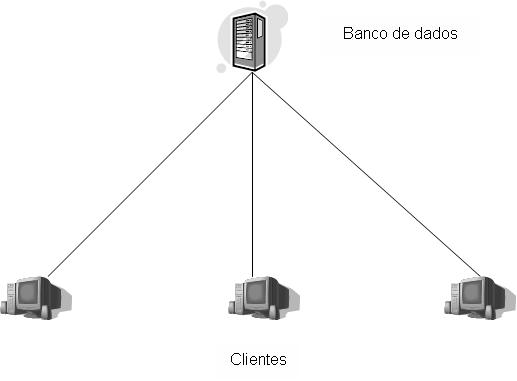
\includegraphics[scale=0.65]{images/cliente-servidor}}\\
Fonte: \cite{devmediaMultiCamadaP12018}
\label{f_c2_cliente_servidor}
\end{figure}

Na camada do cliente, é onde o usuário interage com o sistema, ela é responsável por prover uma \ac{UI} agradável e de fácil acesso para o usuário possa manipular o sistema. Mas apesar de prover a \ac{UI}, a camada do cliente não se restringe a isso, regras de negócio também podem ser implementadas, assim diminuindo a complexidade no servidor. A camada do cliente, de acordo com a sua  complexidade pode ser definida de duas formas ???????????????. Sendo elas:

\begin{itemize}
    \item Cliente Gordo
    \begin{itemize}
        \item Maior complexidade de regras de negócio
        \item Menos processamento para o servidor
        \item Possivelmente mais tráfego na rede
        \item Cliente é mais sensível a mudanças
    \end{itemize}
    \item Cliente Magro
    \begin{itemize}
        \item Menor complexidade de regras de negócio
        \item Mais processamento para o servidor
        \item Menor tráfego na rede
        \item Manutenção mais simples
    \end{itemize}
\end{itemize}

Com o modelo de duas camadas foi possível que \textit{softwares} de terceiros tivessem acesso ao banco de dados, ou seja, com isso os \textit{softwares} poderiam ser diferentes para cada usuário ou setor, afim de melhor atender às suas necessidades. Outra vantagem é a questão do custo-beneficio, as estações dos clientes são mais baratas do que um servidor ???????????????????.

O modelo de duas camadas também pode apresentar algumas desvantagens, como sua aplicação é dividida em partes, acaba acarretando em um \textit{software} mais complexo, com novos cenários a serem tratados. A comunicação do cliente com o servidor se dá por meio da rede, com isso dados sensíveis serão trafegados na rede e precisam de um cuidado maior com a criptografia ???????????????.

\subsection*{Modelo de Multicamadas}
Modelo de multicamadas ou cliente servidor de múltiplas camadas, se consolida a partir dos anos 90 como resposta a  popularização da internet e melhoria das tecnologias de redes, sendo  uma evolução do modelo de duas camadas. Ele tem como propósito  que uma aplicação cliente não realizasse comunicação direta com o banco de dados, no meio do caminho haveria uma ou mais camadas, que elas sim se comunicariam com o banco de dados. A ideia básica é distribuir o processamento da aplicação em várias máquinas, evitando a sobrecarga sobre uma única camada, como ocorria no modelo cliente-servidor. Com a distribuição da carga de processamento em diversas máquinas é possível melhorar o desempenho e compartilhar recursos, utilizando-os como se fossem recursos locais, característica conhecida como  transparência de uso \cite{devmediaMultiCamadaP12018}. Com isso a aplicação pode ser dividida em pequenos pedaços, cada um com sua responsabilidade. Além dessas vantagens, há uma compensação no custo em relação ao desempenho, a possibilidade de aumento de escala e expansão da rede sem perda de qualidade, melhora na robustez em função da distribuição dos serviços em mais de uma máquina, e muitos outros benefícios \cite{devmediaMultiCamadaP12018}.

Em uma aplicação que faz uso do  modelo de multicamadas, faz se necessário ao menos três camadas: camada de apresentação, camada de regras de negócio e a camada de dados. A \autoref{f_c2_multicamada} apresenta o esquema de um sistema multicamada. ?????????????????

\begin{figure}[!htpb]
	\centering
	\caption{Modelo Multicamada}
	\label{f_c2_multicamada}
	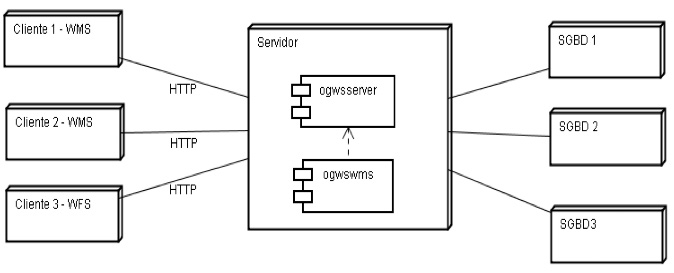
\includegraphics[width=14cm]{images/multicamada.jpg}\\
    Fonte: ?????????????/
 
\end{figure}

\subsection{Camada de Apresentação}

A camada de apresentação fica fisicamente localizada na estação cliente e é responsável por fazer a interação do usuário com o sistema. É uma camada bastante leve, que basicamente executa os tratamentos de telas e campos e geralmente acessa somente a segunda camada, a qual faz as requisições ao banco de dados e devolve o resultado. É também conhecida como cliente, regras de interface de usuário ou camada de interface \cite{devmediaMultiCamada2018}.

\subsection{Camada de Regra de Negócio}

Também conhecida como servidor de aplicação, lógica de negócio ou camada de acesso a dados, essa camada é a responsável por intermediar a comunicação entre a camada de apresentação com a camada de dados, só ela tem acesso a camada de dados. O servidor de aplicação é, geralmente, uma máquina dedicada e com elevados recursos de hardware, uma vez que nele é que ficam armazenados os métodos remotos (regras de negócios) e é realizado todo o seu tratamento e processamento. \cite{devmediaMultiCamada2018}.

\subsection{Camada de Dados}

Também chamada de camada de banco de dados, essa camada é onde se localiza o \ac{SGBD}, ela é responsável por receber requisições da camada de regra de negócio, interpretá las e assim executá-las no banco de dados ???????????????.


\section{Vantagens}

O modelo de multicamadas apresentou diversas vantagens em relação ao modelo de duas camadas, são essas as que mais se destacam:

\subsection{Clientes Leves}

Diferentemente do modelo de duas camadas, onde a regra de negócio era divida tanto na camada do cliente quanto na do servidor, aqui a camada intermediária é quem fica a cargo disso, na camada de apresentação será apenas para visualização de dados, além de possuir possíveis tratamentos de campos e telas ???????????.

\subsection{Facilidade de Redistribuição}

As estações clientes acessam a mesma camada intermediária, sendo assim, quando houver novas implementações ou alterações nas regras de negócios, será refletido para todas as estações clientes ??????????.

\subsection{Modularização}

A modularização refere-se a separar a lógica do negócio e regras de acesso ao banco de dados da camada de apresentação. Desta maneira, várias aplicações clientes podem compartilhar as mesmas regras, que ficam encapsuladas em uma camada de acesso comum.Assim sendo, as regras ficam centralizadas em um único local, ao contrário de em uma aplicação desenvolvida em duas camadas, na qual geralmente existe redundância nestas regras e uma mudança mesmo que pequena acarretará na redistribuição do aplicativo em cada estação cliente \cite{devmediaMultiCamada2018}.

\subsection{Economia de conexões no servidor}

Em um sistema com o modelo de duas camadas, as estações clientes se comunicavam diretamente ao servidor que se localizava o banco de dados, então para cada estação cliente conectada era uma conexão aberta com o banco de dados, sendo que o banco de dados possuí um limite para conexões, tendo isso em vista, no modelo de multicamadas isso não ocorre já que quem se conecta com o banco de dados é o servidor de aplicação, localizado em uma camada intermediária, e uma conexão realizada pelo servidor de aplicação é compartilhada para as estações clientes a ele conectado, sendo assim poderia se ter várias estações clientes requisitando recursos do banco de dados, mas apenas uma conexão estaria aberta já que quem ficaria responsável pela conexão é o servidor de aplicação \cite{devmediaMultiCamada2018}.

\subsection{Independência de localização}

A localização não é um empecilho para a comunicação entre camadas, a estação cliente pode estar fisicamente distante para acessar as camadas intermediárias??????????.

\subsection{Escalabilidade}

No modelo de duas camadas, quando um grande número de estações clientes se conectam ao servidor, acaba ocorrendo uma grande perda de desempenho. Já com o modelo de multicamadas este problema pode ser contornado, já que é possível replicar a regra de negócio em servidores distintos através do balanceamento de carga, isso quer dizer que quando um servidor de aplicação estiver sobrecarregado, outro servidor é acionado para ajudar no controle de conexões, isso também pode ser usado quando um servidor de aplicação parar de funcionar \cite{devmediaMultiCamada2018}.

\section{Estilos Arquitetônicos}

Nesta seção será apresentados os estilos arquitetônicos de desenvolvimento de uma aplicação web.

\subsection{Arquitetura Monolítica}

Segundo \cite{monoVsMicro2017},  "Uma aplicação monolítica é aquele tipo de aplicação na qual toda a base de código está contida em um só lugar, ou seja, todas as funcionalidades estão definidas no mesmo bloco". Esse bloco geralmente se divide em três partes: apresentação, negócio e dados. A \autoref{f_c2_app_monolitica} apresenta o modelo dessa arquitetura.

\begin{figure}[h]
	\centering
	\caption{Aplicação Monolitica}
	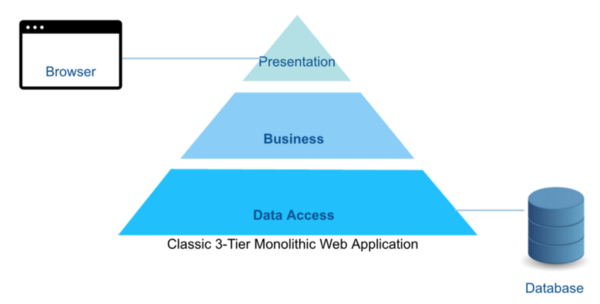
\includegraphics[scale=0.7]{images/app-monolitica.png}\\
	Fonte: ?????????????/
 	\label{f_c2_app_monolitica}
\end{figure}

\newpage
\subsection*{Camadas}

\subsection*{Apresentação}
Camada responsável pela visualização ou interface, que será apresentada para o usuário. "Em uma aplicação web, esta camada contém as páginas \ac{HTML} com \ac{JS} e \ac{CSS} que serão renderizadas no \textit{browser} de quem as acessar",  \cite{monoVsMicro2017}.

\subsection*{Negócio}
Camada que é responsável pela lógica da aplicação. Segundo \cite{monoVsMicro2017} "Nesta camada geralmente se encontram todas as bases de código, chamadas, \ac{API}'s e literalmente toda a inteligência do sistema em questão".

\subsection*{Dados}
Camada em que se encontram as classes encarregadas pela conexão com o \ac{SGBD} ou outro tipo de sistema de armazenamento de dados \cite{monoVsMicro2017}.

\subsection*{Vantagens}
\begin{itemize}
	\item Fácil deploy da aplicação.
	\item Não há duplicidade de código.
	\item Aplicação é desenvolvida usando uma mesma tecnologia.
	\item Seu desenvolvimento tende a ser mais rápido, por ser uma arquitetura mais simples.
	\item Fluxo de deploy simples.
\end{itemize}

\subsection*{Desvantagens}
\begin{itemize}
	\item Ponto único de falha.
	\item Aumento de tamanho e complexidade ao longo do tempo.
	\item Falta de flexibilidade, já que usa uma mesma tecnologia.
	\item Baixa escalabilidade, tendo que copiar toda a aplicação para escalar horizontalmente.
	\item Alta dependência de componentes.
	\item Dificuldade de alterações em produção, qualquer mudança se faz necessário, a reinicialização de todo o sistema.
	\item Demora de aculturamento, um novo desenvolvedor pode ter dificuldades para entender o funcionamento de um componente.
\end{itemize}

\subsection{Arquitetura de Micro serviços}
Uma arquitetura de micro serviços segundo \cite{microservices2014}:  \begin{citacao}"é uma abordagem que desenvolve uma aplicação única como uma suíte de pequenos serviços, cada um rodando em seu próprio processo e se comunicando com mecanismos leves, geralmente uma \ac{API} de recurso \ac{HTTP}" \end{citacao} Desse jeito nós separamos uma aplicação monolítica em pequenas aplicações autônomas, ou seja, devem possuir um sistema de deploy automático e independente, além de que cada aplicação possui um conjunto de regras de negócio específico. A \autoref{f_c2_app_monolitica_vs_microservices} mostra a comparação entre a arquitetura monolítica e de micro serviços.



\begin{figure}[!htpb]
	\centering
	\caption{Representação de módulos monolítico e micro serviços}
	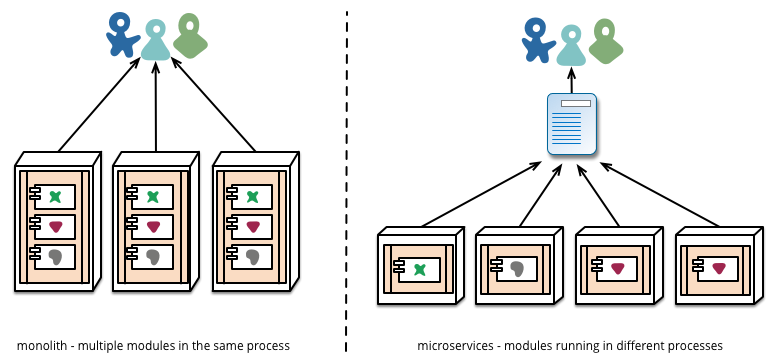
\includegraphics[width=15cm]{images/micro-deployment.png}\\
	Fonte: ??????????????????????/
 	\label{f_c2_app_monolitica_vs_microservices}
\end{figure}

\subsection*{Vantagens}
\begin{itemize}
	\item Arquitetura individual simples.
	\item Sistemas totalmente independentes.
	\item Ausência de ponto de falha única.
	\item Fácil deploy da aplicação e testes unitários.
	\item Módulos podem usar tecnologias distintas.
	\item Serviços coesos e desacoplados.
	\item Facilidade de alterações em ambiente de produção, apenas o serviço específico é necessário ser reinicializado para refletir as alterações.
	\item Escalabilidade do sistema, serviços que sofrem de alta demanda podem ser replicados individualmente.
\end{itemize}

\subsection*{Desvantagens}
\begin{itemize}
	\item Desempenho prejudicado pela latência da rede e pelo custo de serialização e deserialização.
	\item Se a aplicação não for bem documentada, a arquitetura geral tende a ser tornar complexa.
	\item Falta de planejamento e má execução, a arquitetura pode se tornar uma grande bagunça.
	\item Repetição de código nos serviços.
\end{itemize}

%arquiteturas web
% ----------------------------------------------------------------------- %
% Arquivo: cap3.tex
% ----------------------------------------------------------------------- %
\chapter{Arquitetura dos Dispositivos Móveis}
\label{c_cap3}

Atualmente, os dispositivos móveis, são imprescindíveis na vida das pessoas. Quem imaginaria que no começo eles que tinham recursos muito limitados, poucas funcionalidades, se restringindo basicamente a serem calculadoras, e hoje, temos praticamente computadores pessoais em nossas mãos, tanto, em relação a funcionalidades quanto na questão de poder de processamento.

A medida que, os dispositivos móveis foram evoluindo, novas funcionalidades foram aparecendo, calendário, rádio, jogos, mas foi quando a Apple lançou seu primeiro smartphone, o Iphone, com seu próprio \ac{SO} o IOS, e a Google lançou o seu \ac{SO} para smartphones, o Android, que os dispositivos móveis ganhariam a fama de hoje. Com esses sistemas abriu se um leque de oportunidades para empresas e programadores avulsos, à desenvolverem os mais diversos aplicativos.

Com isso em mente, esse capítulo abordará um breve histórico da evolução dos dispositivos móveis, apresentará os \ac{SO}s mais famosos, mostrará como é desenvolver uma aplicação para cada \ac{SO} e analisará as diferenças entre elas.

\section{Evolução dos Dispositivos Móveis}


\section{Android}
\section{iOS}
\section{Comparação entre IOS e Android}




%Arquitetura do MOBILE
\chapter{\Large{\textbf{Conhecendo as Progressives Web Apps}}}

Progressives Web Apps (PWA) é uma tecnologia emergente do Google, um conceito relativamente novo no mundo dos dispositivos móveis e da internet. De acordo com o Google Developers \cite{pwa}: \begin{citacao}
"As Progressive Web Apps fornecem uma experiência instalável, semelhante a um aplicativo, em computadores e dispositivos móveis que são criados e entregues diretamente pela Web. Eles são aplicativos da web que são rápidos e confiáveis. E o mais importante, são aplicativos da web que funcionam em qualquer navegador."
\end{citacao}

 \ac{PWA}s são desenvolvidas usando certas tecnologias e abordagens para criar aplicações que aproveitam os recursos dos dispositivos móveis nativos e de aplicativos da Web, essencialmente é uma mistura de aplicações web e mobiles nativas.

O \cite{pwa} definiu um \textit{checklist} a ser seguido para se considerar uma aplicação como uma \ac{PWA} são elas:

\begin{itemize}
	\item Progressivo - Funciona para qualquer usuário, independentemente do navegador escolhido, pois é criado com aprimoramento progressivo como princípio fundamental.
	\item Responsivo - Se adéqua a qualquer formato: desktop, celular ou tablet.
	\item Independente de conectividade - Aprimorado com \textit{service workers} para trabalhar \textit{off-line} ou em redes de baixa qualidade.
	\item Semelhante a aplicativos - Parece com aplicativos para os usuários, com interações e navegação de estilo de aplicativos, pois é compilado no modelo de \textit{shell} de aplicativo.
	\item Atual - Sempre atualizado graças ao processo de atualização do \textit{service worker}.
	\item Seguro - Fornecido via HTTPS para evitar invasões e garantir que o conteúdo não seja adulterado.
	\item Descobrível - Pode ser identificado como “aplicativo” graças aos manifestos W3C e ao escopo de registro do \textit{service worker}, que permitem que os mecanismos de pesquisa os encontrem.
	\item Reenvolvente - Facilita o reengajamento com recursos como notificações \textit{push}.
	\item Instalável - Permite que os usuários “guardem” os aplicativos mais úteis em suas telas iniciais sem precisar acessar uma loja de aplicativos.
	\item Linkável - Compartilhe facilmente por URL, não requer instalação complexa.
\end{itemize}

\section{Características}
\label{s_c4_caractetisticas}

\subsection{Confiável}
Quando iniciado a partir da tela inicial do usuário, os \textit{service workers} permitem que uma \ac{PWA} seja carregado instantaneamente, independentemente do estado da rede \cite{pwa}.


Basicamente os \textit{service workers} são \textit{scripts} que o navegador roda por debaixo dos panos, separado de uma página Web. Possibilitando que recursos sejam acessados mesmo sem uma interação do usuário ou de uma página Web. O \textit{service worker} possui hoje funcionalidades como \textit{Push Notifications}, que é basicamente, uma notificação que o usuário recebe sem requisita-lá, e Sincronização em Segundo Plano, que é uma \ac{API} que permite que a aplicação adie ações até que o usuário tenha uma conectividade com a internet estável. Isso é útil para garantir que uma ação feita pela o usuário, seja realmente realizada \cite{servicework}.
O \textit{service worker} é uma \ac{API} interessante para os desenvolvedores já que permite configurar experiências off-line. Os S\textit{ervice Workers} possuem algumas características importantes:

\begin{itemize}
	\item É executado em uma \textit{thread} separada do navegador, portanto, não possui acesso ao \ac{DOM} diretamente.
	\item É um \textit{proxy} de rede programável, portanto, permite gerenciar as solicitações de rede da página.
	\item É encerrado quando ficar ocioso e reiniciado quando for necessário.
	\item Os \textit{service workers} utilizam promessas para retornar os dados de suas funções.
\end{itemize}

O \textit{Service Worker} possui um ciclo de vida à parte da página da Web e funciona em uma estrutura já determinada. Entendendo como cada evento ocorre e suas respostas é o ideal para se ter a melhor forma de atualizar e guardar os arquivos. Primeiramente é necessário registrar o service worker na aplicação, isso pode ser feito via um arquivo \ac{JS}, pode se adicionar uma verificação, antes do registro, para verificar se o navegador suporta o uso de \textit{service worker}, após registrar o \textit{service worker} o navegador inicia a etapa de instalação em segundo plano \cite{pwa2}.

Na etapa de instalação, é onde se normalmente é armazenado recursos estáticos em cache. Se todos os recursos forem salvos em cache corretamente, o service worker estará instalado. Se no momento de guardar os recursos, ocorrer alguma falha, a etapa de instalação não será finalizada corretamente, e portanto, o service worker não será ativado. Finalizando a etapa de instalação, é iniciada a fase de ativação, é nesse evento onde se gerencia o cache da aplicação e deleta coisas antigas de versões anteriores \cite{servicework}.

Após a etapa de ativação, o service worker gerenciará as páginas dentro do seu escopo, com exceção da página que registrou o service worker, onde ela só será controlada se for carregada novamente. Enquanto o service worker estiver controlando as páginas, ele poderá assumir dois estados: tratando de eventos de busca e mensagens que as páginas possam gerar, ou encerrado, para economizar memoria do dispositivo \cite{servicework}.


A \autoref{f_c4_sw_ciclo} mostra uma versão minimalista do ciclo de vida do service worker, em sua primeira instalação.

\begin{figure}[!htpb]
	\centering
	\caption{Ciclo de Vida do Service Worker}
	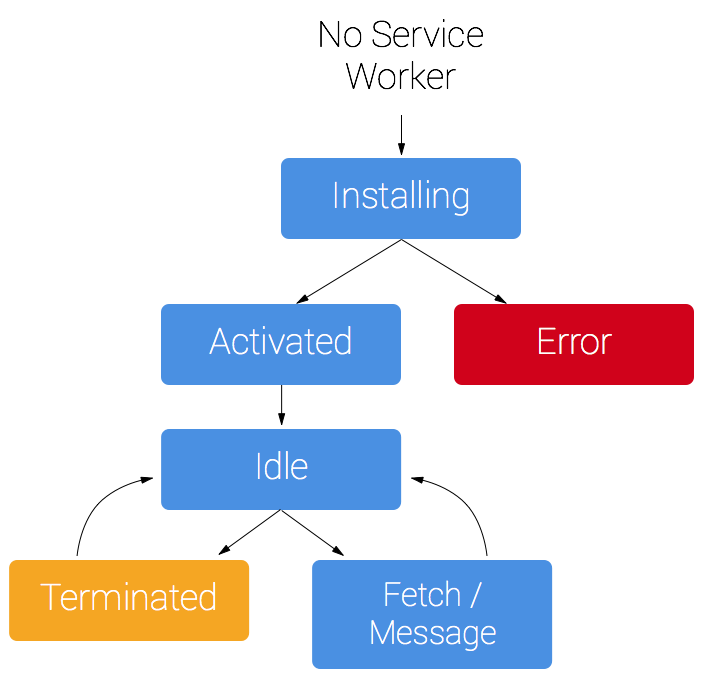
\includegraphics[scale=0.18]{images/sw-lifecycle.png}\\
	{\footnotesize Fonte:\cite{servicework}}
 	\label{f_c4_sw_ciclo}
\end{figure}

\subsection{Rápido}
A maioria dos dados das \ac{PWA}s é salvo no armazenamento do dispositivo no primeiro acesso. A próxima vez que o usuário acessá-la, a aplicação fará o download de poucos dados. Este é um recurso útil para pessoas que possuem conexão com a internet limitada. O aplicativo é mais confiável do que apenas um site e permite que você envie notificações para seus usuários, mesmo depois que o aplicativo for fechado. Uma vez armazenado em um dispositivo, leva muito menos tempo para ser reativo do que um site comum que precisa buscar e carregar tudo de novo \cite{memoir}.

\subsection{Integração e Engajamento}

As \ac{PWA}s são instaláveis e podem ser exibidos na tela inicial do usuário, sem a necessidade de uma loja de aplicativos, como Google Play Store ou Apple Store. Elas oferecem uma experiência imersiva em tela cheia com a ajuda do arquivo de manifesto do aplicativo web.

O Manifesto do Aplicativo Web, é um arquivo no formato \ac{JSON}, que permite controlar como a aplicação irá aparecer e como ela será iniciada, ela conterá também informações relevantes a aplicação, assim fazendo com que o navegador entenda que a aplicação é uma \ac{PWA} e assim o navegador apresentará uma mensagem para o usuário para que se possa instalar o app na tela inicial do \textit{smartphone} \cite{manifest}.

\begin{figure}[!htpb]
	\centering
	\caption{Adicionar a tela inicial}
	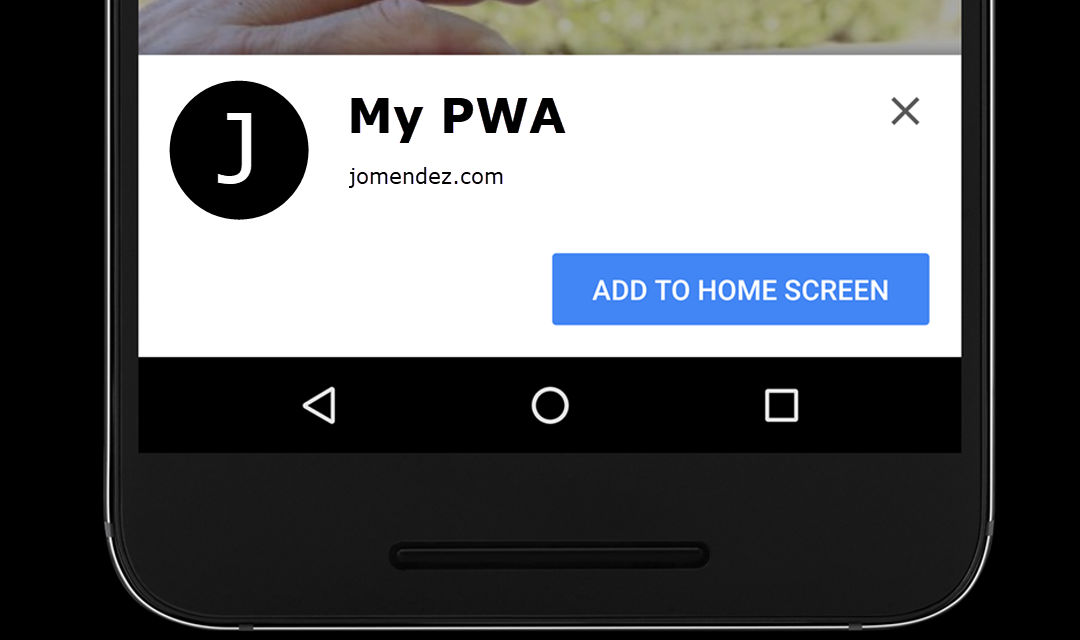
\includegraphics[width=12cm]{images/add-to-home-screen.png}\\
    {\footnotesize Fonte:\cite{pwaHomeScreen}}
 	\label{f_c4_add_home}
\end{figure}

Existem algumas configurações disponíveis no arquivo de manifesto, sendo algumas bem importantes como:

\begin{itemize}
	\item background color - Define a cor de fundo esperada para a aplicação. Esse valor repete o que já está disponível no CSS do site, mas pode ser usado pelos navegadores para desenhar a cor de fundo de um atalho quando o manifesto está disponível antes de a folha de estilo ser carregada. Isso cria uma transição suave entre o carregamento da aplicação e o carregamento do conteúdo do site \cite{manifestfile}.
	\item description - Fornece uma descrição geral do que a aplicação representa
	\item lang - Especifica o idioma principal para as propriedades, "name" e "short name"
	\item dir - Especifica a direção do texto principal para os membros "name", "short name" e "description". Juntamente com o membro "lang", ajuda na exibição correta dos idiomas da direita para a esquerda \cite{manifestfile}.
	\item display - Define o modo de exibição da aplicação.
	\item icons - Especifica uma lista de arquivos de imagem que podem servir como ícones de aplicativo, configurando de acordo com a resolução de tela do dispositivo.
	\item related applications - Define uma lista de aplicativos nativos que podem ser instalados ou acessíveis via plataforma externa, como Google Play Store, esses aplicativos podem ser versões alternativas da aplicação \ac{PWA} \cite{manifestfile}.
	\item short name - Fornece um nome curto legível para o aplicativo. Isso é feito quando não há espaço suficiente para exibir o nome completo da aplicação, como as telas iniciais dos dispositivos.
	\item theme color - Define a cor do tema padrão para a aplicação. Isso às vezes afeta o modo como o sistema operacional o exibe.
\end{itemize}

\section{Vantagens}
\subsection{Fácil Instalação e Atualização}
Como já foi apresentado, para adicionar ou instalar uma aplicação \ac{PWA}, os usuários simplesmente precisam abrir seu site progressivo em um navegador em seu dispositivo móvel. Em algum momento, eles serão solicitados a adicionar o aplicativo em sua tela inicial, ou os usuários podem adicionar o próprio \ac{PWA} no menu do navegador. Bem simples em comparação a aplicativos nativos, em que o usuário necessita ir a uma plataforma de aplicativos e instalar \cite{pwabenefits}.

Quanto às atualizações, os usuários de aplicações \ac{PWA} não precisam atualizar seu aplicativo toda vez que for lançada uma nova versão, eles sempre terão o mais novo.

\subsection{Custos Reduzidos de Desenvolvimento e Suporte}
Não precisa criar uma solução diferente para cada plataforma, pois o mesmo \ac{PWA} funciona no \textit{Android} e no \textit{iOS} e cabe em qualquer dispositivo. Devido à atualização fácil e simultânea, existirá apenas uma versão do aplicativo circulando. O que significa que não se gastará custos extras suportando várias versões \cite{pwabenefits}.

\subsection{Rápido, Leve e Seguro}
Com o \ac{PWA} implementado, a aplicação pode ser carregada em poucos segundos, o que é possível graças aos dados armazenados em cache pelos. Sendo menores em tamanho do que os aplicativos móveis nativos, as \ac{PWA} são mais leves e eficientes e usam menos capacidade e dados do dispositivo. Ao mesmo tempo, eles fornecem uma experiência de usuário próxima à de um aplicativo nativo \textit{Service Workers}. Além disso todas as aplicações \ac{PWA} funcionam via HTTPS, o que significa segurança extra e nenhum acesso não autorizado aos dados \cite{pwa2}.

\subsection{Não necessita de nenhuma loja de aplicativos}
Para publicar uma aplicativo nativo para dispositivo móvel é necessário enviá-lo para alguma loja de aplicativos, como, Google Play Store ou Apple Store, e que ainda vai passar por um processo de análise do aplicativo. Com uma \ac{PWA}, não há necessidade de aguardar o término do período de moderação e como já mencionado, para instalar a aplicação progressiva, os usuários só precisarão abrir o website e clicar em "Adicionar à tela inicial". Embora se comportando como um aplicativo nativo, a \ac{PWA} ainda seria uma página da Web, clicável e compartilhável, e também é indexada pelo Google \cite{pwabenefits}.

\subsection{Customizável}
Se o usuário estiver sem conexão e quiser acessar novas páginas que não foram guardadas em cache, a aplicação não irá travar, mas mostrará uma mensagem personalizada, como na \autoref{f_c4_pwa_scren}:

\begin{figure}[!htpb]
	\centering
	\caption{Telas Customizadas}
	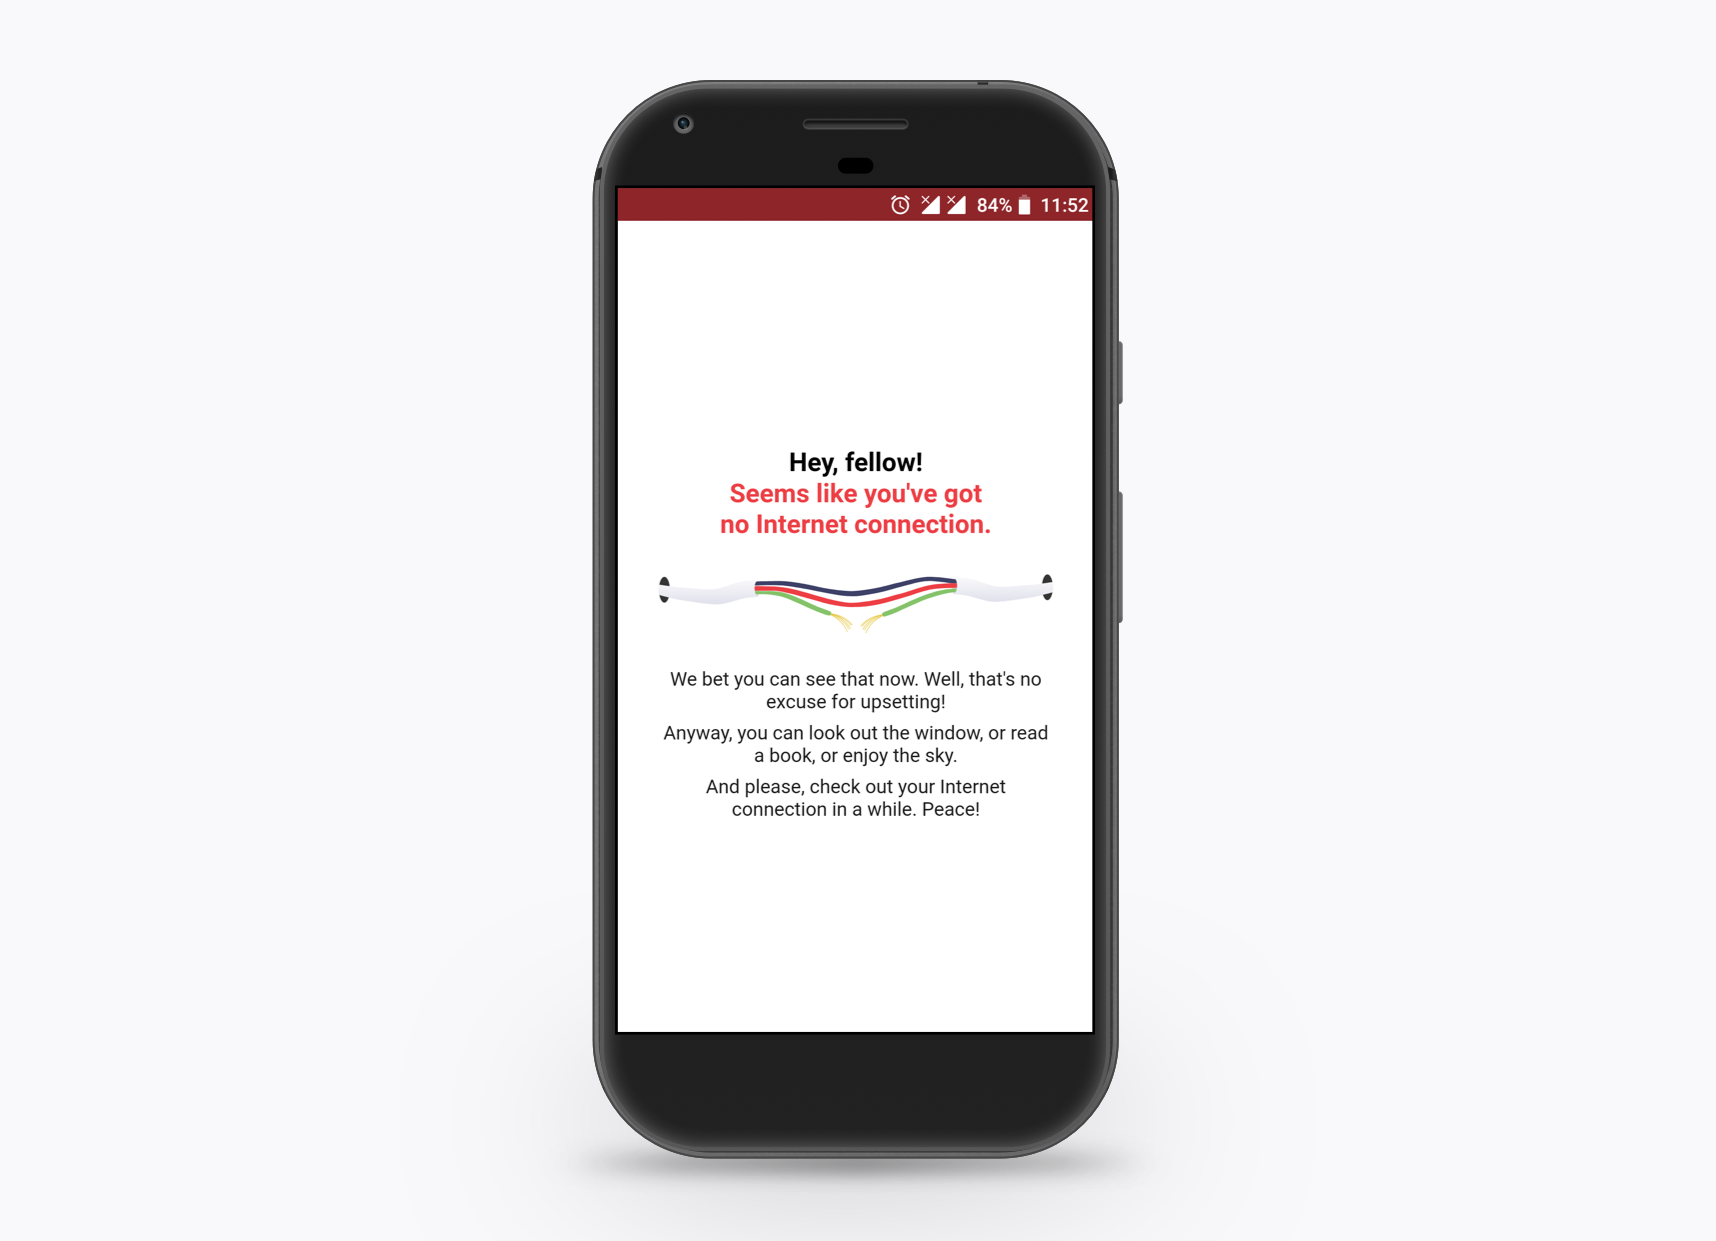
\includegraphics[scale=0.20]{images/pwa_custom.png}\\
	{\footnotesize Fonte:\cite{pwabenefits}}
 	\label{f_c4_pwa_scren}
\end{figure}

\section{Desvantagens}
\subsection{Funcionalidades Limitadas}
As \ac{PWA} ainda são sites e ainda não suportam todas as funcionalidades que os aplicativos nativos podem oferecer. Elas têm acesso limitado a recursos dos dispositivos. Além disso, as \ac{PWA} podem oferecer um nível de notificação menos personalizado se comparado aos aplicativos nativos.

\subsection{Limitações para o iOS}
No momento, ainda há uma lacuna entre as \ac{PWA} para Android e iOS. Embora os PWAs estejam disponíveis para usuários do iOS, nem todos os recursos que funcionam em dispositivos Android são oferecidos para iOS, no entanto, existe um movimento na equipe por trás do iOS que aos poucos estão implementando recursos para serem usados via \ac{PWA}, e provavelmente os usuários do iOS irão receber as mesmas funcionalidades das aplicações progressivas disponíveis no Android \cite{pwaios}.%Introdução ao PWA
\chapter{Análise comparativa entre PWAs e Aplicações Móveis Nativas}

As \ac{PWA}s provaram ser muito úteis, e foram apresentados diversos recursos disponíveis em dispositivos móveis, em que as \ac{PWA}s dão suporte. No entanto, eles não estão aqui para tomar o lugar dos aplicativos nativos, mas para corrigir alguns problemas, como a compatibilidade entre plataformas e funcionamento em baixa conectividade e até mesmo offline.

Tendo isso em vista, esse capítulo irá abordar, o que são as aplicações para dispositivos móveis nativas, e uma comparação levando em consideração as vantagens e desvantagens entre desenvolver uma aplicação \ac{PWA} e um aplicativo nativo.

\section{Aplicação Nativa}
Os aplicativos nativos são desenvolvidos para um dispositivo específico ou uma plataforma, como Android e iOS, e podem interagir e aproveitar os recursos fornecidos por esse dispositivo específico. Esses aplicativos oferecem acesso mais rápido a diferentes recursos do dispositivo, como câmera, microfone, agenda, localização e etc.
Para usa-lós é necessário realizar a instalação do aplicativo no dispositivo desejado, normalmente os aplicativos se encontram nas lojas das plataformas, mas também é possível instalar via pacotes externos \cite{native}.

Ao desenvolver uma aplicação nativa, é necessário muitas vezes usar linguagens de programação específicas para a plataforma, elas permitem ao desenvolvedor ter acesso às funcionalidades de \ac{API} e hardware do dispositivo. As linguagens de programação disponíveis para desenvolver aplicativos nativos, varia para cada plataforma \cite{native}. Abaixo alguns exemplos das linguagens de programação disponíveis:

\begin{itemize}
	\item Java - Linguagem oficial do sistema operacional Android, usado para criar aplicativos nativos para a plataforma.
	\item Kotlin - Linguagem mais recente e semelhante ao Java, também para criar aplicativos nativos para Android.
	\item Objective-C - Linguagem principal para criar \textit{software} para dispositivos iOS.
	\item Swift -  Linguagem lançada da Apple para a criação de \textit{software} para o iOS, propõe-se a ser mais simples de implementar do que o Objective-C.
\end{itemize}

\section{Comparativo PWA e Aplicação nativa}
\subsection{Criação da aplicação e Distribuição}
\subsection*{Aplicação Nativa}
O desenvolvimento de uma aplicação móvel nativa para Android e iOS requer duas equipes, uma para cada sistema. Mesmo que os aplicativos de ambos os sistemas sejam desenvolvidos ao mesmo tempo, ainda demorará mais para garantir que a funcionalidade seja a mesma para os dois aplicativos. Tudo isso significa tempo e custos consideráveis necessários para criar um aplicativo.

O envio e aprovação via App Stores é uma parte separada da distribuição do aplicativo móvel nativo. O produto terá que passar por um período de moderação, pela equipe da plataforma, o que geralmente leva algum tempo. Para a Google Play Store, pode levar algumas horas, enquanto na Apple App Store pode levar de dois a quatro dias. Esse tempo de moderação, acaba impactando no atraso da distribuição da aplicação.

\subsection*{PWA}
A criação de uma \ac{PWA} requer apenas uma equipe de desenvolvimento da Web, pois na verdade é um site, embora com alguns recursos nativos dos dispositivos móveis. A validação pelas lojas não é necessária, pois se está criando um \textit{website}. Não é necessário enviar a aplicação para nenhuma loja nem esperar que ele seja aprovado. Depois que a \ac{PWA} é construída e publicada na Web, ela está pronto para ser usada.

\subsection{Instalação}
\subsection*{Aplicação Nativa}
Basicamente o fluxo de instalação é, ir em uma loja de aplicativos, procurar a aplicação e realizar o download, e após isso, a instalação no dispositivo móvel, e por fim o aplicativo estará disponível para uso.

\subsection*{PWA}
Com a \ac{PWA} é necessário abrir um navegador, acessar o site da aplicação, irá ser apresentado uma mensagem, perguntando se quer adicionar a aplicação para a tela inicial do dispositivo, confirmando, a aplicação irá ser instalada.

\subsection{Engajamento do Usuário}
Uma das ferramentas de engajamento mais poderosas é a \textit{Push Notifications}. São mensagens entregues por meio de um aplicativo instalado nos dispositivos, nos dispositivos móveis ou nos desktops dos usuários, para alertar seus usuários sobre novas chegadas de ações, vendas ou outras notícias.

\subsection*{Aplicação Nativa}
Em aplicativos móveis nativos, a disponibilidade do recurso de notificações por \textit{push} não depende do sistema operacional ou do modelo do dispositivo. Os usuários os receberão independentemente desses fatores.

\subsection*{PWA}
Nas \ac{PWA}, as \textit{Push Notifications} também estão disponíveis, mas apenas para o Android. Isso é possível graças aos \textit{service workers} eles podem enviar notificações quando uma aplicação \ac{PWA} não está em execução.

\subsection{Funcionamento Offline}
\subsection*{Aplicação Nativa}
Quando estamos falando sobre o modo offline do aplicativo nativo, assumimos que ele opera da mesma maneira que na conexão. O ponto é que um aplicativo nativo mostra o conteúdo e a funcionalidade que ele conseguiu armazenar em \textit{cache} quando a conexão ainda estava lá. Isso está disponível devido ao armazenamento local e à sincronização suave de dados com a nuvem.

\subsection*{PWA}
Nas aplicações \ac{PWA}, os usuários também podem aproveitar o modo offline. Quando ativadas, as páginas mostram o conteúdo pré-carregado ou carregado, que é fornecido com os \textit{service workers}. No entanto, o modo offline nas \ac{PWA}s é um pouco mais lento em comparação a um aplicativo móvel nativo, pois ele é implementado de forma diferente. Ao mesmo tempo, a diferença entre os dois tipos de aplicativos não é tão drástica.%Estudo Comparativo (Tabela evidenciando a diferença MOBILE x WEB x PWA)
\chapter{Estudo de Caso}%Estudo de Caso
\chapter{Conclusão}% Conclusao
% ----------------------------------------------------------
% PARTE I
% ----------------------------------------------------------
%\part{Preparação da pesquisa}

% Capitulo com exemplos de comandos inseridos de arquivo externo 
%\chapter{Fundamentação Teórica}\label{fundamentacao}
Nesta seção será apresentado os conceitos necessários para um completo entendimento deste trabalho. A \autoref{gerenciadeconfiguracao} aborda os conceitos inerentes à gerência de configuração, juntamente com algumas ferramentas CASE (Computer-Aided Software Engineering), com ênfase em Integração Contínua descrito na \autoref{integracaocont} e por fim na \autoref{processonpi} será descrito o processo do NPI e uma ênfase no processo de Gerência de Configuração.

\section{Gerência de Configuração}\label{gerenciadeconfiguracao}
\section{Gerência de Configuração}\label{gerenciadeconfiguracao}
A gerência de configuração é a área da engenharia de software responsável pela evolução do software. Ela atua durante todo o ciclo de vida do produto de software e, por meio de técnicas, ferramentas e metodologias, visa garantir que as mudanças que irão ocorrer dentro do ciclo de vida do desenvolvimento do software sejam identificadas, avaliadas e comunicada a todos os envolvidos através de ferramentas que auxiliam neste processo de evolução.
Portanto "o propósito do processo de Gerência de Configuração é estabelecer e manter a integridade de todos os produtos de trabalho de um processo ou projeto e disponibilizá-la a todos os envolvidos"\space\cite{mpsbr}.
\subsection{Plano de Gerenciamento de Configuração}\label{pgc}
O Plano de Gerenciamento de Configuração (PGC) descreve todas as atividades de configuração e mudança que serão realizadas durante o projeto. Um conjunto de atividades, responsabilidades, ferramentas, recursos e etc. A gerência de configuração tem como objetivo garantir a integridade dos itens de configuração, que são quaisquer artefatos que estejam sob custódia da gerência de configuração, através do versionamento, da identificação e controle de mudanças e acesso \cite{pressman2010}. 

\subsection{Sistema de Controle de Versão}
Um sistema de controle de versão: "	[...] combina procedimentos e ferramentas para gerenciar diferentes versões de objetos de configurações que são criadas durante o processo de engenharia de software" \cite[p.~927]{pressman2010}.
Atualmente, o uso de sistemas de controle de versão se tornou comum nas empresas de grande e pequeno porte. Tais ferramentas permitem que se tenha o controle de diferentes versões de arquivos que estão submetidos ao versionamento, recuperação de versões antigas, visualização de alterações realizadas em arquivos e saber por quem, e quando o arquivo foi alterado. Através de comandos (i.e.,\textit{check-in},\textit{check-out}) os usuários conseguem se comunicar com o repositório a fim de obter os artefatos ali armazenados \cite{gleiph2011}.

Em situações especiais, faz-se necessário que os desenvolvedores trabalhem em uma linha diferente da original chamada de \textit{mainline} geralmente essa situação ocorre quando tem-se como objetivo a correção de \textit{bugs} de versões anteriores do repositório, nesse caso, um \textit{branch}, uma ramificação na linha de desenvolvimento do controle de versão, é criado afim de permitir a realização desta ação, concedendo assim o trabalho em paralelo sobre o mesmo repositório.
\begin{figure}[h]
\centering
\caption[Branch no Sistema de Controle de Versão]{Branch no Sistema de Controle de Versão.}
\includegraphics[width=0.5\linewidth]{./images/branch}
\label{fig:Branch}
\legend {\fontsize{10}{12}\selectfont {Fonte: \citeonline{tableless2012}}.}
\end{figure}
A \autoref{fig:Branch} demonstra a criação de um \textit{branch} paralelo à linha de desenvolvimento principal chamada de branch feature1 e branch master respectivamente. Posteriormente as ações realizadas no \textit{branch feature1} são incorporadas ao \textit{branch master}.

Os sistemas de controle de versão podem possuir três características: Local, Centralizado e Distribuído. Um sistema de controle de versão local armazena todas as informações de um arquivo submetido ao versionamento na máquina, localmente, guardando diferentes versões daquele arquivo. Enquanto um sistema de controle de versão centralizado como o nome diz, possui um único servidor centralizado, como o \textit{subversion} \footnote{http://subversion.apache.org}, \textit{perforce} \footnote{http://www.perforce.com} este tipo de padrão de SCV mantém em seu único servidor todos os arquivos versionados. Para cada comando de comunicação realizado nos arquivos versionados, uma requisição deverá ser feita, podendo gerar lentidão ou deixar o servidor fora de funcionamento. E por fim os sistemas de controle de versão distribuídos que possuem um servidor central onde os arquivos são submetidos ao versionamento, entretanto, cada desenvolvedor possui em sua máquina de trabalho as versões que estavam no servidor, tornando cada \textit{workstation} um "servidor", portanto, caso ocorra um problema no servidor central, estes podem ser recuperados via \textit{workstation}, mantendo assim, a integridade dos arquivos e evitando ser um ponto único de falha \cite{git}	.


\subsection{Sistema de Controle de Mudança}
Todo software sofre mudanças enfrentar essas mudanças é o papel da gerência de configuração, e para isso o gerente de configuração utiliza um sistema de controle de mudança. "O controle de mudança combina procedimentos humanos e ferramentas automatizadas para proporcionar um mecanismo de controle de mudança"\space \citeonline[p~.930]{pressman2010}. As mudanças devem ser avaliadas com cautela baseando-se, em seu custo benefício. Uma combinação de esforço e \textit{business value}. A mudança tem início quando um "cliente" solicita a mudanças através de um formulário, conhecido como \textit{change request}.

 Nesse formulário está descrito os aspectos da mudança. Após a solicitação ser realizada, esta deve ser avaliada, verificando se a mesma já foi solicitada, ou corrigida em caso de \textit{bugs}. Após a mudança ser validada, uma equipe de desenvolvedores avaliam os impactos que esta mudança tem sobre o sistema, verificando custo/benefício e esforço de realização \cite{sommerville2011}. Posterior a esta análise, a mudança será avaliada por um comitê de controle de mudança (CCB), que avaliará o impacto da perspectiva do negócio, que decidirá se esta mudança será revisada, aprovada ou reprovada. Alguns sistemas que fornecem este controle sobre as mudança são: \textit{Redmine \footnote{http://www.redmine.org}, GitHub \footnote{http://www.github.com} Jira \footnote{https://www.atlassian.com/software/jira}}
\subsection{Auditoria de Configuração}
"Uma auditoria de configuração de software complementa a revisão técnica formal ao avaliar um objeto de configuração quanto às características que geralmente não são consideradas durante a revisão"\space\citeonline[p~.934]{pressman2010}. Ela tem como objetivo garantir que mesmo com as mudanças realizadas no software, a qualidade foi mantida. As auditorias se dividem em dois tipos: auditorias funcionais e auditorias físicas, a auditoria física baseia-se em verificar se os itens de configuração estão devidamente atualizados e se as práticas e padrões foram realizados da maneira correta, enquanto a auditoria funcional busca verificar os aspectos lógicos dos itens de configuração.
\subsection{Ferramentas de Build}
As ferramentas de \textit{build} têm como objetivo automatizar processos repetitivos, aumentando a produtividade e facilitando o trabalho do desenvolvedor. Através da definição de uma rotina, ou conjunto de comandos, o desenvolvedor informa a ferramenta que tipo de processo ele deseja automatizar, podendo ser uma compilação, teste de classe, recriação de uma tabela nova no banco de dados, comprimir arquivos css e javascript. Cabe ao desenvolvedor definir o escopo da automatização. Alguns exemplo deste tipo de ferramenta são: \textit{Ant, Grunt, Gulp, Maven}.


\begin{figure}[H]
\centering
\caption[Processo Lógico de uma Build]{Processo Lógico de uma Build.}
\includegraphics[scale=0.7]{./images/build}
\label{fig:build}
\legend {\fontsize{10}{12}\selectfont {Fonte: \citeonline{paul2007}}.}
\end{figure}
Na figura \autoref{fig:build} um \textit{script} foi definido para realizar as seguintes funções: \textit{clean} no projeto, compilação do código fonte, integração com o banco de dados, execução dos testes, inspeções no código e por fim,o \textit{deploy} da aplicação.


%\subsection{Ferramentas de Integração Contínua}

\section{Integração Contínua}\label{integracaocont}
\begin{OnehalfSpace}
A integração contínua tem como objetivo identificar erros mais rapidamente, permitindo que alterações efetuadas e integradas aos repositórios dos sistemas de controle de versão sejam posteriormente verificadas e, caso erros ocorram, estes sejam notificados imediatamente ao autor da alteração.
A melhor definição acerca de integração contínua foi definida por \citeonline{fowler2000}
\end{OnehalfSpace}

\begin{citacao}
"[...] uma prática de desenvolvimento de software onde os membros de um time integram seu trabalho frequentemente, geralmente cada pessoa integra pelo menos diariamente – podendo haver múltiplas integrações por dia. Cada integração é verificada por uma \textit{build} automatizada (incluindo testes) para detectar erros de integração o mais rápido possível. Muitos times acham que essa abordagem leva a uma significante redução nos problemas de integração e permite que um time desenvolva software coeso mais rapidamente." \citeonline[tradução nossa]{fowler2000}.
\end{citacao}

\subsection{Características de Integração}
Os requisitos para utilização de uma ferramenta de integração contínua de acordo com \citeonline{Anti2010} são:
\begin{itemize}
\item {\textbf{Uma conexão com um sistema de controle de versão:}}

A integração contínua necessita desta conexão, pois ela identifica as alterações ocorridas no repositório, e inicia o processo de integração.

\item {\textbf{A definição de uma \textit{build}:}}

A integração contínua possui uma \textit{build} privada que será executada assim que o processo de integração for iniciado, e é esta \textit{build} que definirá quais ações serão realizadas no processo de integração, tais como compilação, testes, análise de código.
\item {\textbf{Um mecanismo de \textit{feedback}:}}

Um dos principais objetivos da integração contínua consiste em seu \textit{feedback} imediato, sendo assim, um mecanismo deste tipo é essencial para a ferramenta, tais como e-mail, sms.
\item {\textbf{Um processo de integração do código: }}
O processo de integração consiste em como este será realizado, se manualmente ou através de um servidor de integração contínua.

\end{itemize}

\subsection{Processo de Integração}
A integração ocorre quando alguma mudança é enviada ao sistema de controle de versão do repositório, que, através de um servidor de integração contínua identifica as mudanças e executa sua \textit{build} privada \cite{mraz2013}. 


\begin{figure}[H]
\centering
\caption[Ambiente de Integração Contínua]{Ambiente de Integração Contínua.}
\includegraphics[scale=1.0]{./images/CI}
\label{fig:CI}
\legend {\fontsize{10}{12}\selectfont Fonte: \citeonline{paul2005}.}
\end{figure}

A \autoref{fig:CI} descreve um ambiente em que um servidor de integração contínua é utilizado. Existem três ambientes de trabalho distintos formado por três desenvolvedores, que obtiveram uma cópia do projeto do repositório do SCV para trabalharem em suas \textit{workstation}. Durante o trabalho, alterações foram efetuadas e foi realizado o \textit{commit} ao repositório central. Após a inserção junto ao repositório, o servidor de integração contínua verifica as alterações e executa uma \textit{build} de integração. Caso exista um problema com a \textit{build} e esta não seja bem sucedida, o responsável pela alteração será informado sobre o ocorrido, assim seu objetivo em diante será a correção da \textit{build}.

\subsection{Benefícios da Integração Contínua}

Esta subseção tem como objetivo destacar os principais objetivos existentes na utilização de uma ferramenta de integração contínua.

As principais vantagens em utilizar um servidor de integração contínua segundo \citeonline[p.~29]{paul2007} são:

\begin{itemize}
\item {\textbf{Redução de Riscos}}: 
Através da detecção imediada de código quebrados, ou incorretos, reduz-se riscos atrelados ao produto.
\item {\textbf{Redução de processos manuais repetitivos}}:
Um conjunto de tarefas são executadas automaticamente pela build privada do servidor de integração contínua.
\item {\textbf{Permitir melhor visibilidade do projeto}}:
Através da identificação de informações inerentes ao desenvolvimento, como frequência de códigos defeituosos, módulos mais complexos, permitindo maior gerenciamento do projeto.
\item {\textbf{Estabelecer uma maior confiança no produto do time de desenvolvimento}}:
Através da visualizações de mudanças bem sucedidas, os desenvolvedores sentem maior confiança ao realizarem mudanças.

\item\textbf{Coleta de métricas a cada \textit{build}}: Um dos benefícios que podem ser obtidos através da ferramenta, é a coleta das métricas do código a ser desenvolvido e alterado. Através da utilização de uma ferramenta de análise estática de código é possível realizar uma análise de violações, não conformidades. E por meio desses indicadores, a equipe consegue ter um maior controle no desenvolvimento do software, investindo na melhoria contínua do software.
\end{itemize}	

%\subsection{Integração Contínua e a Redução de Riscos}
%Os Riscos em produtos de software estão diretamente relacionados. Segundo \citeonline[p~.48]{paul2007} se você consegue reduzir certos riscos no software, você pode melhorar a qualidade do software.
%\subsection{Builds Automatizadas}
%Builds são rotinas de execução definidas com o objetivo de reduzir processos repetitivos. Durante o processo de desenvolvimento de um software muitas ações tendem a serem repetidas por parte dos desenvolvedores, utilizar o tempo para a realização  de atividades que poderiam ser automatizadas, de forma manual, reduz a produtividade e preocupações com melhorias devido ao tempo "apertado". Somando-se a isso, uma build garante que tudo que está nela definido será executado, evitando assim, que determinada ação seja esquecida, ou caso um novo membro entre na equipe uma explicação do que ele deve fazer, ou não esquecer de fazer, não faz-se necessário.

\subsection{Integração Contínua Manual}
Na integração contínua manual o processo de integração é realizado individualmente, possibilitando que apenas um desenvolvedor realize \textit{check-in} no repositório durante o intervalo de integração \citeonline{gleiph2011}. Este tipo de abordagem permite que apenas uma pessoa realize o \textit{check-in}, assim, as integrações serão contínuas e seguidas, não paralelas. Este tipo de abordagem garante uma maior confiabilidade nas integrações, pois segue um padrão de integração e os itens do repositório possuem maior consistência, garantindo que a estrutura do repositório seja mantida \cite{gleiph2011}.

\subsection{Integração Contínua Automatizada}
A integração contínua automatizada é auxiliada pelo uso de um servidor de integração contínua, que obtém do controle de versão as alterações realizadas e executa sua \textit{build} privada com o objetivo de verificar possíveis erros gerados por essas modificações.
\begin{citacao}
Integração contínua automática possui a vantagem de ser escalável e, deste  modo, oferecer  maior  suporte  ao  trabalho  colaborativo.  Com  a utilização de Servidores de IC, a responsabilidade  de realizar construções da integração é retirada  dos desenvolvedores. Portanto, os desenvolvedores podem realizar \textit{check-in} sem a necessidade de conquistar a vez de integrar. Esse fator é fundamental para que os  \textit{check-ins}  continuem sendo verificados sem a necessidade de um desenvolvedor realizar a construção e identificar problemas, resultando na eliminação do gargalo humano. \citeonline[p~.54]{gleiph2011}. 
\end{citacao}

\subsection{Processo de Escolha da Ferramenta}\label{escolhaFerramenta}
Esta seção define um conjunto de características que auxiliam no processo de escolha de uma ferramenta de integração contínua.
\begin{itemize}
\item {\textbf{Suporte à Linguagem:}}

O processo de escolha de um servidor de integração continua deve ser baseado de acordo com o suporte a linguagem, visto que alguns sistemas são construídos para trabalharem com uma linguagem de programação específica.

\item {\textbf{Suporte ao Sistema de Controle de Versão:}}

Como explanado anteriormente, a importância do SCV dentro de um servidor de integração contínua é altíssima, portanto escolher uma ferramenta que integre-se com o repositório é essencial, pois alguns servidores fornecem suporte a SCV mais populares, como \textit{Subversion}, \textit{Git}, entretanto pode não haver suporte ao \textit{Mercurial} por exemplo.


\item {\textbf{Segurança:}}

Garantir que somente pessoas autorizadas devem ter acessos aos artefatos existentes no servidor de integração contínua.

\item {\textbf{Extensibilidade:}}

Capacidade da ferramenta ter funcionalidades adicionadas por meio de \textit{plugins}, ser extensível.

\item {\textbf{Usabilidade:}}

Possuir baixa dificuldade na realização de ações dentro da ferramenta, boa aprendizagem, compreensibilidade.

\item {\textbf{Instalação e Configuração:}}

Facilidade de instalação em diferentes ambientes de operação, tais como sistemas operacionais, hardware através da utilização de recursos. Documentação clara e objetiva do processo de instalação.


\end{itemize}


\section{Métricas de Software}

Uma métrica de software é uma característica de um determinado sistema de software, desenvolvimento, processo ou documentação, de modo que possa ser medido \cite{sommerville2011}.

As métricas de software são dados quantitativos que informaram o estado de um sistema de software. Através desses dados, é possível um maior controle e tomada de decisão pela parte gerencial de uma organização de software \cite{karina2008}. São exemplos de métricas segundo \citeonline{merson2014}:
\begin{itemize}
\item{Cobertura de Testes}
\item{Complexidade Ciclomática}
\item{Débito Técnico}
\end{itemize}	

Dentre o conjunto de métricas avaliados, as violações estão inseridas. Violações são não conformidades encontradas em um conjunto de regras definidas.

As violações podem ser classificadas em diferentes graus de severidade:

\begin{itemize}
\item{Critical:} Causam perda de dados, vulnerabilidades de segurança, tornam o sistema inutilizável.
\item{Major: Erros que impactam uma minoria de usuários do sistema.}
\item{Normal: Erros que afetam uma parte da funcionalidade do sistema.}
\item{Minor: Estão mais relacionados ao estilo do código.}
\end{itemize}	


\section{Processo do NPI}\label{processonpi}
O NPI possui um modelo de processo definido, este processo é baseado nos modelos e metodologias Scrum, MPS.BR e XP. Este modelo define as práticas e o modelo de trabalho dos envolvidos nas atividades do núcleo. Dentro do modelo de processo definido no NPI \footnote{http://www.npi.quixada.ufc.br/processo/} este trabalho tem como objetivo focar no modelo de processo de gerência de configuração.

O NPI subdivide-se em dois turnos, manhã e tarde, sendo cada turno supervisionado por um professor supervisor diferente. Estes turnos podem ou não estar trabalhando no mesmo projeto, embora o mais comum é que trabalhem em projetos diferentes. As equipes contam com em média oito membros onde comumente destes, dois são alocados para as atividades de requisitos e testes, um para liderança técnica, enquanto o restante da equipe é alocado para as atividades de desenvolvimento, incluindo o líder técnico. O professor supervisor tem como papel o auxílio aos líderes técnicos, acompanhamento do projeto, avaliação dos estagiários, escolha dos projetos a serem desenvolvidos pelas equipes e usualmente realizar o papel de \textit{Product Owner}. 

O líder técnico possui papel gerencial bem como de desenvolvimento, suas atribuições partem desde a condução de reuniões, resolução de conflitos,atribuição e definições de tarefas, até o acompanhamento das atividades. 

A \autoref{fig:processo-npi} mostra o processo utilizado no NPI modelado através da ferramenta EPF Composer. Na figura	existem duas atividades que ocorrem em paralelo, são elas: Avaliação do Processo e Iniciar Projeto, este que subdivide-se em mais três atividades, a primeira delas a atividade de Requisitos, que posteriormente fornece entrada para um ciclo de \textit{Sprints} que ocorrerá enquanto houver funcionalidades não implementadas, simultaneamente com a atividade de Requisitos estão de Gerenciamento do Projeto e o Gerenciamento de Configuração.
\begin{figure}[H]
\centering
\caption[Processo do NPI]{Processo do NPI.}
\includegraphics[scale=0.8]{./images/processo-npi}
\label{fig:processo-npi}
\legend {\fontsize{10}{12}\selectfont {Fonte: \citeonline{processonpi}}.}
\end{figure}


\subsection{Processo de Gerência de Configuração do NPI}
O modelo de processo\footnote{http://www.npi.quixada.ufc.br/processo/} relacionado a gerência de configuração é descrito na \autoref{fig:procnpi}. Este modelo de processo possui duas atividades que serão descritas abaixo:
\begin{itemize}
\item \textbf{Criar Plano de Gerenciamento de Configuração:} Esta atividade é realizada pelo líder técnico da equipe envolvida. Esta atividade subdivide-se em quatro etapas são elas:
\begin{itemize}
\item \textbf{Identificar Itens de Configuração:} Esta atividade caracteriza-se pela criação, especificação e seleção dos produtos de trabalho, ferramentas, itens que tem objetivo descrever os produtos de trabalho. Exemplos de itens desta atividade são: Requisitos, Diagramas, Testes.

\item \textbf{Atribuir Identificadores únicos para os itens de configuração:} Esta atividade possui um nome bem sugestivo tem como intuito atribuir a cada item de configuração um identificador único de modo a facilitar a identificação dentro do projeto. O identificador segue o padrão $\left[PROJETO\right]$-$\left[TIPO\right]$-EXTRA.EXTENSÃO. Como exemplo um artefato possuiria o seguinte identificador: $\left[GPA\right]$-$\left[REQ\right]$-Especificacao.doc

\item \textbf{Identificar o responsável por cada item de configuração:} Esta atividade tem como objetivo atribuir a cada item de configuração um responsável, permitindo assim, uma maior facilidade na identificação do responsável de um determinado item de configuração.
\item \textbf{Criar	Plano de Gerenciamento de Configuração:} Esta atividade tem como objetivo a elaboração do PGC explicado na \autoref{pgc} por meio dos dados obtidos com as tarefas anteriores. O plano define os responsáveis pelas atividades de Gerência de Configuração, ferramentas e ambientes a serem utilizados e todos os itens de configuração identificados.
\end{itemize}
\item \textbf{Estabelecer um sistema de Gestão de Configuração:} Esta atividade tem como requisito que o plano de gerenciamento de configuração esteja concluído, e possui apenas uma etapa:
\begin{itemize}
\item \textbf{Estabelecer um sistema de Gestão de Configuração:} Esta atividade tem como objetivo definir as ferramentas de acesso, ambiente de armazenamento e métodos para criação e alteração dos itens de configuração \cite{processonpi}. 
\end{itemize}
\end{itemize}

\begin{figure}[H]
\centering
\caption[Processo de Gerenciamento de Configuração]{Processo de Gerenciamento de Configuração.}
\includegraphics[scale=1.3]{./images/processonpi}
\label{fig:procnpi}
\legend {\fontsize{10}{12}\selectfont Fonte: \citeonline{processonpi}.}
\end{figure}


%\chapter{Trabalhos Relacionados}\label{trabalhorel}
Nesta seção será descrito trabalhos que influenciaram os conceitos envolvidos neste trabalho, além de demonstrar pontos comuns e distintos entre si e o proposto.

O trabalho de \citeonline{pereira2013} descreve a implantação de uma ferramenta de integração contínua em um departamento de desenvolvimento e pesquisa, o Sedna, de uma empresa de engenharia, em um ambiente de MPS.BR nível F. Onde os principais clientes do Sedna são voltados a área de óleo e gás.

Durante o período de implantação, o Sedna fornecia manutenção a três sistemas, onde um tratava-se de uma aplicação web, deste modo o \textit{deploy} da aplicação para todos os seus usuários era de responsabilidade do Sedna. Tal ação tornava-se bastante custosa devido ao grande número de web sites que deveriam ser atualizados.
	
Dentro do Sedna algumas ferramentas de gerência de configuração já eram utilizadas, tais como o Atlassian Jira, Subversion (SVN) e o Atlassian Confluence. Ainda com a utilização destas ferramentas a equipe possuía grandes dificuldades no tempo de realização do \textit{deploy}, pois esta atividade consumia uma grande parte do tempo da equipe, tempo de aprendizagem e realização do \textit{deploy} da aplicação, principalmente para novos membros da equipe, e um \textit{feedback} atrasado para problemas básicos de commits errôneos.

Os autores descrevem que os pontos positivos da integração estão a utilização de uma ferramenta de integração contínua da mesma empresa que fornecia o sistema de gerenciamento de projetos, a ferramenta utilizada foi o Atlassian Bamboo e a utilização de ferramentas de automação do processo de build, o que facilitava o trabalho da integração contínua. Bem como o autor destaca as experiências negativas da implantação, que estão na ausência de uma máquina com requisitos mínimos exigidos para a utilização, a ausência de treinamento da equipe, onde os conhecimentos de IC estavam com o líder de projetos e o gerente de configuração, e por fim a ferramenta não fornecia suporte ao \textit{redeploy} dos artefatos gerados, o que gerou uma barreira na equipe acerca da ferramenta.


Uma das principiais vantagens da utilização da integração contínua é o seu \textit{feedback} imediato acerca de problemas de integração, e, entender e interpretar as principais causas dos problemas de integração foi realizado por \citeonline{miller2008}. Quando este percebeu que em um projeto da Microsoft, o Service Factory, a maior causa de falha na build eram violações no sistema de análise de código seguido por testes automatizados e erros de compilação.

A obtenção de métricas através da coleta contínua de métricas é uma grande vantagem incluída dentro da integração contínua, pois a sua principal vantagem é o aumento da qualidade do produto ao facilitar o processo de manutenção do software. Para isso \citeonline{moreira2010} desenvolveram um \textit{framework} para a extração de métricas automatizadas, implementado em um ambiente de integração contínua, logo, evidenciou-se a importância das inspeções e teste de códigos nas \textit{builds}, como foi descrito anteriormente.

Os testes são fundamentais na qualidade do software, e na confiança do produto em uma \textit{build} de integração contínua. Assim \citeonline{kim2009} propuseram a criação de um \textit{framework} automatizado de testes que permitisse facilitar a  construção dos casos de testes, reuso de componentes, relatórios mais legíveis e integrado ao ambiente de integração contínua.

Implantar uma integração contínua em um ambiente de desenvolvimento ágil foi realizado por \citeonline{abdul2012}. Estes propuseram um conjunto de boas práticas e coletaram experiências acerca desta implantação. Estes afirmam que os engenheiros podem não ser tão facilmente convencidos de aceitar a integração contínua, independentemente se esta é implementada \textit{top-down}, quando parte de uma hierarquia mais elevada da organização para as camadas inferiores, ou \textit{bottom-up}, quando parte dos desenvolvedores até os níveis mais altos da hierarquia, e que em ambas as abordagens existem prós e contras.

%%% abtex2-modelo-include-comandos.tex, v-1.9.2 laurocesar
%% Copyright 2012-2014 by abnTeX2 group at http://abntex2.googlecode.com/ 
%%
%% This work may be distributed and/or modified under the
%% conditions of the LaTeX Project Public License, either version 1.3
%% of this license or (at your option) any later version.
%% The latest version of this license is in
%%   http://www.latex-project.org/lppl.txt
%% and version 1.3 or later is part of all distributions of LaTeX
%% version 2005/12/01 or later.
%%
%% This work has the LPPL maintenance status `maintained'.
%% 
%% The Current Maintainer of this work is the abnTeX2 team, led
%% by Lauro César Araujo. Further information are available on 
%% http://abntex2.googlecode.com/
%%
%% This work consists of the files abntex2-modelo-include-comandos.tex
%% and abntex2-modelo-img-marca.pdf
%%

% ---
% Este capítulo, utilizado por diferentes exemplos do abnTeX2, ilustra o uso de
% comandos do abnTeX2 e de LaTeX.
% ---
 
\chapter{Resultados de comandos}\label{cap_exemplos}

\chapterprecis{Isto é uma sinopse de capítulo. A ABNT não traz nenhuma
normatização a respeito desse tipo de resumo, que é mais comum em romances 
e livros técnicos.}\index{sinopse de capítulo}

% ---
\section{Codificação dos arquivos: UTF8}
% ---

A codificação de todos os arquivos do \abnTeX\ é \texttt{UTF8}. É necessário que
você utilize a mesma codificação nos documentos que escrever, inclusive nos
arquivos de base bibliográficas |.bib|.

% ---
\section{Citações diretas}
\label{sec-citacao}
% ---

\index{citações!diretas}Utilize o ambiente \texttt{citacao} para incluir
citações diretas com mais de três linhas:

\begin{citacao}
As citações diretas, no texto, com mais de três linhas, devem ser
destacadas com recuo de 4 cm da margem esquerda, com letra menor que a do texto
utilizado e sem as aspas. No caso de documentos datilografados, deve-se
observar apenas o recuo \cite[5.3]{NBR10520:2002}.
\end{citacao}

Use o ambiente assim:

\begin{verbatim}
\begin{citacao}
As citações diretas, no texto, com mais de três linhas [...] deve-se observar
apenas o recuo \cite[5.3]{NBR10520:2002}.
\end{citacao}
\end{verbatim}

O ambiente \texttt{citacao} pode receber como parâmetro opcional um nome de
idioma previamente carregado nas opções da classe (\autoref{sec-hifenizacao}). Nesse
caso, o texto da citação é automaticamente escrito em itálico e a hifenização é
ajustada para o idioma selecionado na opção do ambiente. Por exemplo:

\begin{verbatim}
\begin{citacao}[english]
Text in English language in italic with correct hyphenation.
\end{citacao}
\end{verbatim}

Tem como resultado:

\begin{citacao}[english]
Text in English language in italic with correct hyphenation.
\end{citacao}

\index{citações!simples}Citações simples, com até três linhas, devem ser
incluídas com aspas. Observe que em \LaTeX as aspas iniciais são diferentes das
finais: ``Amor é fogo que arde sem se ver''.

% ---
\section{Notas de rodapé}
% ---

As notas de rodapé são detalhadas pela NBR 14724:2011 na seção 5.2.1\footnote{As
notas devem ser digitadas ou datilografadas dentro das margens, ficando
separadas do texto por um espaço simples de entre as linhas e por filete de 5
cm, a partir da margem esquerda. Devem ser alinhadas, a partir da segunda linha
da mesma nota, abaixo da primeira letra da primeira palavra, de forma a destacar
o expoente, sem espaço entre elas e com fonte menor
\citeonline[5.2.1]{NBR14724:2011}.}\footnote{Caso uma série de notas sejam
criadas sequencialmente, o \abnTeX\ instrui o \LaTeX\ para que uma vírgula seja
colocada após cada número do expoente que indica a nota de rodapé no corpo do
texto.}\footnote{Verifique se os números do expoente possuem uma vírgula para
dividi-los no corpo do texto.}. 


% ---
\section{Tabelas}
% ---

\index{tabelas}A \autoref{tab-nivinv} é um exemplo de tabela construída em
\LaTeX.

\begin{table}[htb]
\ABNTEXfontereduzida
\caption[Níveis de investigação]{Níveis de investigação.}
\label{tab-nivinv}
\begin{tabular}{p{2.6cm}|p{6.0cm}|p{2.25cm}|p{3.40cm}}
  %\hline
   \textbf{Nível de Investigação} & \textbf{Insumos}  & \textbf{Sistemas de Investigação}  & \textbf{Produtos}  \\
    \hline
    Meta-nível & Filosofia\index{filosofia} da Ciência  & Epistemologia &
    Paradigma  \\
    \hline
    Nível do objeto & Paradigmas do metanível e evidências do nível inferior &
    Ciência  & Teorias e modelos \\
    \hline
    Nível inferior & Modelos e métodos do nível do objeto e problemas do nível inferior & Prática & Solução de problemas  \\
   % \hline
\end{tabular}
\legend{Fonte: \citeonline{van86}}
\end{table}

Já a \autoref{tabela-ibge} apresenta uma tabela criada conforme o padrão do
\citeonline{ibge1993} requerido pelas normas da ABNT para documentos técnicos e
acadêmicos.

\begin{table}[htb]
\IBGEtab{%
  \caption{Um Exemplo de tabela alinhada que pode ser longa
  ou curta, conforme padrão IBGE.}%
  \label{tabela-ibge}
}{%
  \begin{tabular}{ccc}
  \toprule
   Nome & Nascimento & Documento \\
  \midrule \midrule
   Maria da Silva & 11/11/1111 & 111.111.111-11 \\
  \midrule 
   João Souza & 11/11/2111 & 211.111.111-11 \\
  \midrule 
   Laura Vicuña & 05/04/1891 & 3111.111.111-11 \\
  \bottomrule
\end{tabular}%
}{%
  \fonte{Produzido pelos autores.}%
  \nota{Esta é uma nota, que diz que os dados são baseados na
  regressão linear.}%
  \nota[Anotações]{Uma anotação adicional, que pode ser seguida de várias
  outras.}%
  }
\end{table}


% ---
\section{Figuras}
% ---

\index{figuras}Figuras podem ser criadas diretamente em \LaTeX,
como o exemplo da \autoref{fig_circulo}.

\begin{figure}[htb]
	\caption{\label{fig_circulo}A delimitação do espaço}
	\begin{center}
	    \setlength{\unitlength}{5cm}
		\begin{picture}(1,1)
		\put(0,0){\line(0,1){1}}
		\put(0,0){\line(1,0){1}}
		\put(0,0){\line(1,1){1}}
		\put(0,0){\line(1,2){.5}}
		\put(0,0){\line(1,3){.3333}}
		\put(0,0){\line(1,4){.25}}
		\put(0,0){\line(1,5){.2}}
		\put(0,0){\line(1,6){.1667}}
		\put(0,0){\line(2,1){1}}
		\put(0,0){\line(2,3){.6667}}
		\put(0,0){\line(2,5){.4}}
		\put(0,0){\line(3,1){1}}
		\put(0,0){\line(3,2){1}}
		\put(0,0){\line(3,4){.75}}
		\put(0,0){\line(3,5){.6}}
		\put(0,0){\line(4,1){1}}
		\put(0,0){\line(4,3){1}}
		\put(0,0){\line(4,5){.8}}
		\put(0,0){\line(5,1){1}}
		\put(0,0){\line(5,2){1}}
		\put(0,0){\line(5,3){1}}
		\put(0,0){\line(5,4){1}}
		\put(0,0){\line(5,6){.8333}}
		\put(0,0){\line(6,1){1}}
		\put(0,0){\line(6,5){1}}
		\end{picture}
	\end{center}
	\legend{Fonte: os autores}
\end{figure}

Ou então figuras podem ser incorporadas de arquivos externos, como é o caso da
\autoref{fig_grafico}. Se a figura que ser incluída se tratar de um diagrama, um
gráfico ou uma ilustração que você mesmo produza, priorize o uso de imagens
vetoriais no formato PDF. Com isso, o tamanho do arquivo final do trabalho será
menor, e as imagens terão uma apresentação melhor, principalmente quando
impressas, uma vez que imagens vetorias são perfeitamente escaláveis para
qualquer dimensão. Nesse caso, se for utilizar o Microsoft Excel para produzir
gráficos, ou o Microsoft Word para produzir ilustrações, exporte-os como PDF e
os incorpore ao documento conforme o exemplo abaixo. No entanto, para manter a
coerência no uso de software livre (já que você está usando \LaTeX e \abnTeX),
teste a ferramenta \textsf{InkScape}\index{InkScape}
(\url{http://inkscape.org/}). Ela é uma excelente opção de código-livre para
produzir ilustrações vetoriais, similar ao CorelDraw\index{CorelDraw} ou ao Adobe
Illustrator\index{Adobe Illustrator}. De todo modo, caso não seja possível
utilizar arquivos de imagens como PDF, utilize qualquer outro formato, como
JPEG, GIF, BMP, etc. Nesse caso, você pode tentar aprimorar as imagens
incorporadas com o software livre \textsf{Gimp}\index{Gimp}
(\url{http://www.gimp.org/}). Ele é uma alternativa livre ao Adobe
Photoshop\index{Adobe Photoshop}.

\begin{figure}[htb]
	\caption{\label{fig_grafico}Gráfico produzido em Excel e salvo como PDF}
	\begin{center}
	    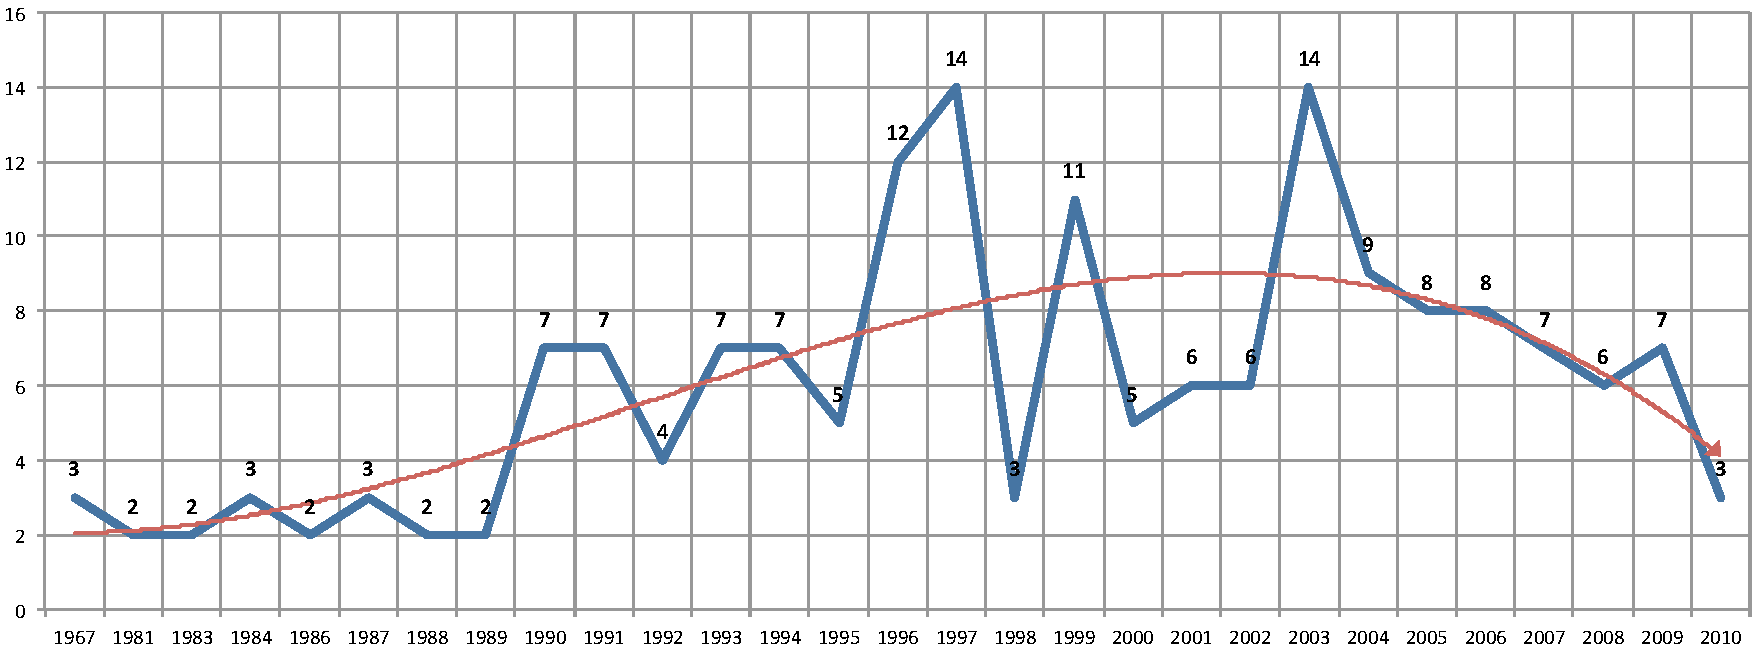
\includegraphics[scale=0.5]{abntex2-modelo-img-grafico.pdf}
	\end{center}
	\legend{Fonte: \citeonline[p. 24]{araujo2012}}
\end{figure}

% ---
\subsection{Figuras em \emph{minipages}}
% ---

\emph{Minipages} são usadas para inserir textos ou outros elementos em quadros
com tamanhos e posições controladas. Veja o exemplo da
\autoref{fig_minipage_imagem1} e da \autoref{fig_minipage_grafico2}.

\begin{figure}[htb]
 \label{teste}
 \centering
  \begin{minipage}{0.4\textwidth}
    \centering
    \caption{Imagem 1 da minipage} \label{fig_minipage_imagem1}
    
\includegraphics[scale=0.9]{abntex2-modelo-img-marca.pdf}
    \legend{Fonte: Produzido pelos autores}
  \end{minipage}
  \hfill
  \begin{minipage}{0.4\textwidth}
    \centering
    \caption{Grafico 2 da minipage} \label{fig_minipage_grafico2}
    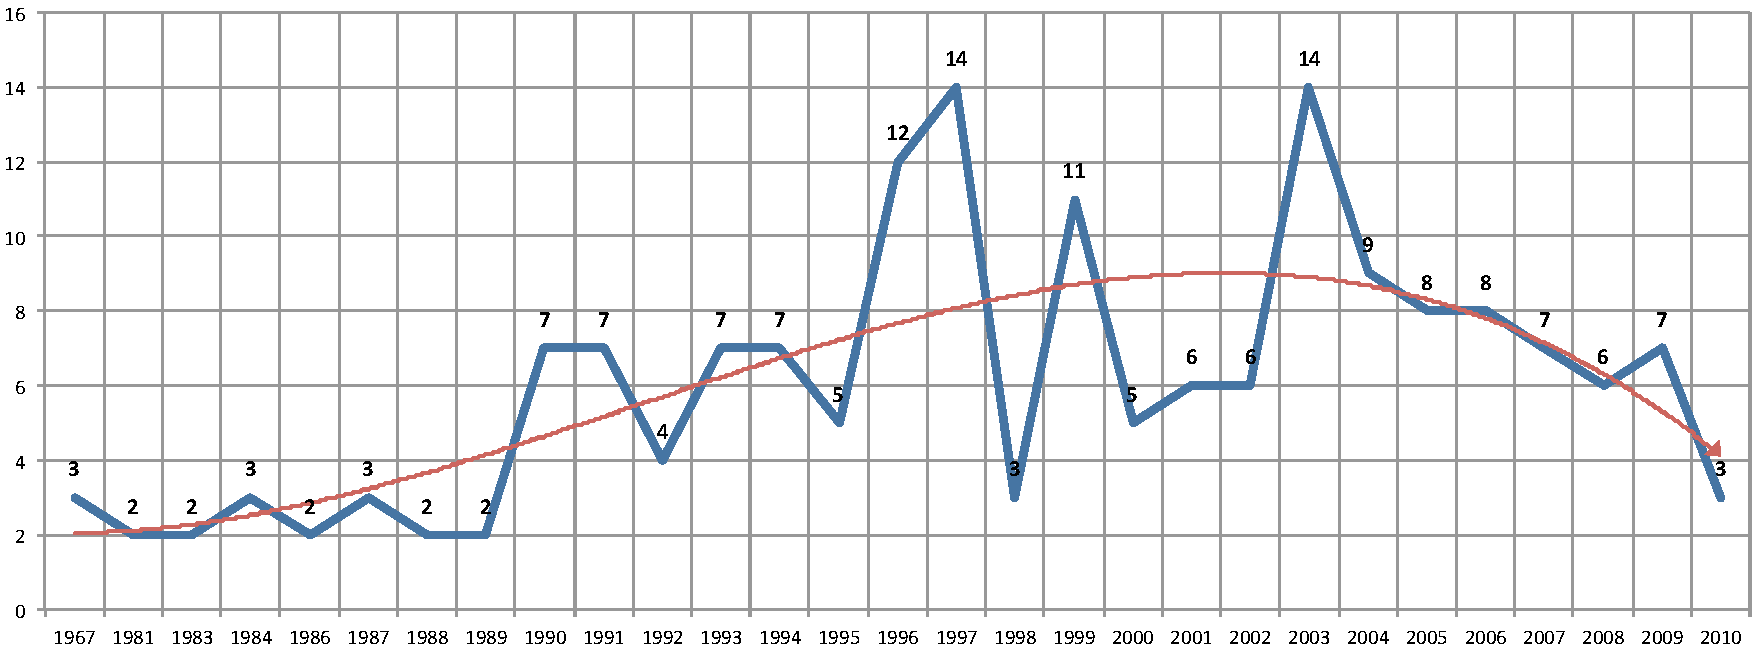
\includegraphics[scale=0.2]{abntex2-modelo-img-grafico.pdf}
    \legend{Fonte: \citeonline[p. 24]{araujo2012}}
  \end{minipage}
\end{figure}

Observe que, segundo a \citeonline[seções 4.2.1.10 e 5.8]{NBR14724:2011}, as
ilustrações devem sempre ter numeração contínua e única em todo o documento:

\begin{citacao}
Qualquer que seja o tipo de ilustração, sua identificação aparece na parte
superior, precedida da palavra designativa (desenho, esquema, fluxograma,
fotografia, gráfico, mapa, organograma, planta, quadro, retrato, figura,
imagem, entre outros), seguida de seu número de ordem de ocorrência no texto,
em algarismos arábicos, travessão e do respectivo título. Após a ilustração, na
parte inferior, indicar a fonte consultada (elemento obrigatório, mesmo que
seja produção do próprio autor), legenda, notas e outras informações
necessárias à sua compreensão (se houver). A ilustração deve ser citada no
texto e inserida o mais próximo possível do trecho a que se
refere. \cite[seções 5.8]{NBR14724:2011}
\end{citacao}

% ---
\section{Expressões matemáticas}
% ---

\index{expressões matemáticas}Use o ambiente \texttt{equation} para escrever
expressões matemáticas numeradas:

\begin{equation}
  \forall x \in X, \quad \exists \: y \leq \epsilon
\end{equation}

Escreva expressões matemáticas entre \$ e \$, como em $ \lim_{x \to \infty}
\exp(-x) = 0 $, para que fiquem na mesma linha.

Também é possível usar colchetes para indicar o início de uma expressão
matemática que não é numerada.

\[
\left|\sum_{i=1}^n a_ib_i\right|
\le
\left(\sum_{i=1}^n a_i^2\right)^{1/2}
\left(\sum_{i=1}^n b_i^2\right)^{1/2}
\]

Consulte mais informações sobre expressões matemáticas em
\url{https://code.google.com/p/abntex2/wiki/Referencias}.

% ---
\section{Enumerações: alíneas e subalíneas}
% ---

\index{alíneas}\index{subalíneas}\index{incisos}Quando for necessário enumerar
os diversos assuntos de uma seção que não possua título, esta deve ser
subdividida em alíneas \cite[4.2]{NBR6024:2012}:

\begin{alineas}

  \item os diversos assuntos que não possuam título próprio, dentro de uma mesma
  seção, devem ser subdivididos em alíneas; 
  
  \item o texto que antecede as alíneas termina em dois pontos;
  \item as alíneas devem ser indicadas alfabeticamente, em letra minúscula,
  seguida de parêntese. Utilizam-se letras dobradas, quando esgotadas as
  letras do alfabeto;

  \item as letras indicativas das alíneas devem apresentar recuo em relação à
  margem esquerda;

  \item o texto da alínea deve começar por letra minúscula e terminar em
  ponto-e-vírgula, exceto a última alínea que termina em ponto final;

  \item o texto da alínea deve terminar em dois pontos, se houver subalínea;

  \item a segunda e as seguintes linhas do texto da alínea começa sob a
  primeira letra do texto da própria alínea;
  
  \item subalíneas \cite[4.3]{NBR6024:2012} devem ser conforme as alíneas a
  seguir:

  \begin{alineas}
     \item as subalíneas devem começar por travessão seguido de espaço;

     \item as subalíneas devem apresentar recuo em relação à alínea;

     \item o texto da subalínea deve começar por letra minúscula e terminar em
     ponto-e-vírgula. A última subalínea deve terminar em ponto final, se não
     houver alínea subsequente;

     \item a segunda e as seguintes linhas do texto da subalínea começam sob a
     primeira letra do texto da própria subalínea.
  \end{alineas}
  
  \item no \abnTeX\ estão disponíveis os ambientes \texttt{incisos} e
  \texttt{subalineas}, que em suma são o mesmo que se criar outro nível de
  \texttt{alineas}, como nos exemplos à seguir:
  
  \begin{incisos}
    \item \textit{Um novo inciso em itálico};
  \end{incisos}
  
  \item Alínea em \textbf{negrito}:
  
  \begin{subalineas}
    \item \textit{Uma subalínea em itálico};
    \item \underline{\textit{Uma subalínea em itálico e sublinhado}}; 
  \end{subalineas}
  
  \item Última alínea com \emph{ênfase}.
  
\end{alineas}

% ---
\section{Espaçamento entre parágrafos e linhas}
% ---

\index{espaçamento!dos parágrafos}O tamanho do parágrafo, espaço entre a margem
e o início da frase do parágrafo, é definido por:

\begin{verbatim}
   \setlength{\parindent}{1.3cm}
\end{verbatim}

\index{espaçamento!do primeiro parágrafo}Por padrão, não há espaçamento no
primeiro parágrafo de cada início de divisão do documento
(\autoref{sec-divisoes}). Porém, você pode definir que o primeiro parágrafo
também seja indentado, como é o caso deste documento. Para isso, apenas inclua o
pacote \textsf{indentfirst} no preâmbulo do documento:

\begin{verbatim}
   \usepackage{indentfirst}      % Indenta o primeiro parágrafo de cada seção.
\end{verbatim}

\index{espaçamento!entre os parágrafos}O espaçamento entre um parágrafo e outro
pode ser controlado por meio do comando:

\begin{verbatim}
  \setlength{\parskip}{0.2cm}  % tente também \onelineskip
\end{verbatim}

\index{espaçamento!entre as linhas}O controle do espaçamento entre linhas é
definido por:

\begin{verbatim}
  \OnehalfSpacing       % espaçamento um e meio (padrão); 
  \DoubleSpacing        % espaçamento duplo
  \SingleSpacing        % espaçamento simples	
\end{verbatim}

Para isso, também estão disponíveis os ambientes:

\begin{verbatim}
  \begin{SingleSpace} ...\end{SingleSpace}
  \begin{Spacing}{hfactori} ... \end{Spacing}
  \begin{OnehalfSpace} ... \end{OnehalfSpace}
  \begin{OnehalfSpace*} ... \end{OnehalfSpace*}
  \begin{DoubleSpace} ... \end{DoubleSpace}
  \begin{DoubleSpace*} ... \end{DoubleSpace*} 
\end{verbatim}

Para mais informações, consulte \citeonline[p. 47-52 e 135]{memoir}.

% ---
\section{Inclusão de outros arquivos}\label{sec-include}
% ---

É uma boa prática dividir o seu documento em diversos arquivos, e não
apenas escrever tudo em um único. Esse recurso foi utilizado neste
documento. Para incluir diferentes arquivos em um arquivo principal,
de modo que cada arquivo incluído fique em uma página diferente, utilize o
comando:

\begin{verbatim}
   \include{documento-a-ser-incluido}      % sem a extensão .tex
\end{verbatim}

Para incluir documentos sem quebra de páginas, utilize:

\begin{verbatim}
   \input{documento-a-ser-incluido}      % sem a extensão .tex
\end{verbatim}

% ---
\section{Compilar o documento \LaTeX}
% ---

Geralmente os editores \LaTeX, como o
TeXlipse\footnote{\url{http://texlipse.sourceforge.net/}}, o
Texmaker\footnote{\url{http://www.xm1math.net/texmaker/}}, entre outros,
compilam os documentos automaticamente, de modo que você não precisa se
preocupar com isso.

No entanto, você pode compilar os documentos \LaTeX usando os seguintes
comandos, que devem ser digitados no \emph{Prompt de Comandos} do Windows ou no
\emph{Terminal} do Mac ou do Linux:

\begin{verbatim}
   pdflatex ARQUIVO_PRINCIPAL.tex
   bibtex ARQUIVO_PRINCIPAL.aux
   makeindex ARQUIVO_PRINCIPAL.idx 
   makeindex ARQUIVO_PRINCIPAL.nlo -s nomencl.ist -o ARQUIVO_PRINCIPAL.nls
   pdflatex ARQUIVO_PRINCIPAL.tex
   pdflatex ARQUIVO_PRINCIPAL.tex
\end{verbatim}

% ---
\section{Remissões internas}
% ---

Ao nomear a \autoref{tab-nivinv} e a \autoref{fig_circulo}, apresentamos um
exemplo de remissão interna, que também pode ser feita quando indicamos o
\autoref{cap_exemplos}, que tem o nome \emph{\nameref{cap_exemplos}}. O número
do capítulo indicado é \ref{cap_exemplos}, que se inicia à
\autopageref{cap_exemplos}\footnote{O número da página de uma remissão pode ser
obtida também assim:
\pageref{cap_exemplos}.}.
Veja a \autoref{sec-divisoes} para outros exemplos de remissões internas entre
seções, subseções e subsubseções.

O código usado para produzir o texto desta seção é:

\begin{verbatim}
Ao nomear a \autoref{tab-nivinv} e a \autoref{fig_circulo}, apresentamos um
exemplo de remissão interna, que também pode ser feita quando indicamos o
\autoref{cap_exemplos}, que tem o nome \emph{\nameref{cap_exemplos}}. O número
do capítulo indicado é \ref{cap_exemplos}, que se inicia à
\autopageref{cap_exemplos}\footnote{O número da página de uma remissão pode ser
obtida também assim:
\pageref{cap_exemplos}.}.
Veja a \autoref{sec-divisoes} para outros exemplos de remissões internas entre
seções, subseções e subsubseções.
\end{verbatim}

% ---
\section{Divisões do documento: seção}\label{sec-divisoes}
% ---

Esta seção testa o uso de divisões de documentos. Esta é a
\autoref{sec-divisoes}. Veja a \autoref{sec-divisoes-subsection}.

\subsection{Divisões do documento: subseção}\label{sec-divisoes-subsection}

Isto é uma subseção. Veja a \autoref{sec-divisoes-subsubsection}, que é uma
\texttt{subsubsection} do \LaTeX, mas é impressa chamada de ``subseção'' porque
no Português não temos a palavra ``subsubseção''.

\subsubsection{Divisões do documento: subsubseção}
\label{sec-divisoes-subsubsection}

Isto é uma subsubseção.

\subsubsection{Divisões do documento: subsubseção}

Isto é outra subsubseção.

\subsection{Divisões do documento: subseção}\label{sec-exemplo-subsec}

Isto é uma subseção.

\subsubsection{Divisões do documento: subsubseção}

Isto é mais uma subsubseção da \autoref{sec-exemplo-subsec}.


\subsubsubsection{Esta é uma subseção de quinto nível}\label{sec-exemplo-subsubsubsection}

Esta é uma seção de quinto nível. Ela é produzida com o seguinte comando:

\begin{verbatim}
\subsubsubsection{Esta é uma subseção de quinto
nível}\label{sec-exemplo-subsubsubsection}
\end{verbatim}

\subsubsubsection{Esta é outra subseção de quinto nível}\label{sec-exemplo-subsubsubsection-outro}

Esta é outra seção de quinto nível.


\paragraph{Este é um parágrafo numerado}\label{sec-exemplo-paragrafo}

Este é um exemplo de parágrafo nomeado. Ele é produzida com o comando de
parágrafo:

\begin{verbatim}
\paragraph{Este é um parágrafo nomeado}\label{sec-exemplo-paragrafo}
\end{verbatim}

A numeração entre parágrafos numeradaos e subsubsubseções são contínuas.

\paragraph{Esta é outro parágrafo numerado}\label{sec-exemplo-paragrafo-outro}

Esta é outro parágrafo nomeado.

% ---
\section{Este é um exemplo de nome de seção longo. Ele deve estar
alinhado à esquerda e a segunda e demais linhas devem iniciar logo abaixo da
primeira palavra da primeira linha}
% ---

Isso atende à norma \citeonline[seções de 5.2.2 a 5.2.4]{NBR14724:2011} 
 e \citeonline[seções de 3.1 a 3.8]{NBR6024:2012}.

% ---
\section{Diferentes idiomas e hifenizações}
\label{sec-hifenizacao}
% ---

Para usar hifenizações de diferentes idiomas, inclua nas opções do documento o
nome dos idiomas que o seu texto contém. Por exemplo (para melhor
visualização, as opções foram quebras em diferentes linhas):

\begin{verbatim}
\documentclass[
	12pt,
	openright,
	twoside,
	a4paper,
	english,
	french,
	spanish,
	brazil
	]{abntex2}
\end{verbatim}

O idioma português-brasileiro (\texttt{brazil}) é incluído automaticamente pela
classe \textsf{abntex2}. Porém, mesmo assim a opção \texttt{brazil} deve ser
informada como a última opção da classe para que todos os pacotes reconheçam o
idioma. Vale ressaltar que a última opção de idioma é a utilizada por padrão no
documento. Desse modo, caso deseje escrever um texto em inglês que tenha
citações em português e em francês, você deveria usar o preâmbulo como abaixo:

\begin{verbatim}
\documentclass[
	12pt,
	openright,
	twoside,
	a4paper,
	french,
	brazil,
	english
	]{abntex2}
\end{verbatim}

A lista completa de idiomas suportados, bem como outras opções de hifenização,
estão disponíveis em \citeonline[p.~5-6]{babel}.

Exemplo de hifenização em inglês\footnote{Extraído de:
\url{http://en.wikibooks.org/wiki/LaTeX/Internationalization}}:

\begin{otherlanguage*}{english}
\textit{Text in English language. This environment switches all language-related
definitions, like the language specific names for figures, tables etc. to the other
language. The starred version of this environment typesets the main text
according to the rules of the other language, but keeps the language specific
string for ancillary things like figures, in the main language of the document.
The environment hyphenrules switches only the hyphenation patterns used; it can
also be used to disallow hyphenation by using the language name
`nohyphenation'.}
\end{otherlanguage*}

Exemplo de hifenização em francês\footnote{Extraído de:
\url{http://bigbrowser.blog.lemonde.fr/2013/02/17/tu-ne-tweeteras-point-le-vatican-interdit-aux-cardinaux-de-tweeter-pendant-le-conclave/}}:

\begin{otherlanguage*}{french}
\textit{Texte en français. Pas question que Twitter ne vienne faire une
concurrence déloyale à la traditionnelle fumée blanche qui marque l'élection
d'un nouveau pape. Pour éviter toute fuite précoce, le Vatican a donc pris un
peu d'avance, et a déjà interdit aux cardinaux qui prendront part au vote
d'utiliser le réseau social, selon Catholic News Service. Une mesure valable
surtout pour les neuf cardinaux – sur les 117 du conclave – pratiquants très
actifs de Twitter, qui auront interdiction pendant toute la période de se
connecter à leur compte.}
\end{otherlanguage*}

Pequeno texto em espanhol\footnote{Extraído de:
\url{http://internacional.elpais.com/internacional/2013/02/17/actualidad/1361102009_913423.html}}:

\foreignlanguage{spanish}{\textit{Decenas de miles de personas ovacionan al pontífice en su
penúltimo ángelus dominical, el primero desde que anunciase su renuncia. El Papa se
centra en la crítica al materialismo}}.

O idioma geral do texto por ser alterado como no exemplo seguinte:

\begin{verbatim}
  \selectlanguage{english}
\end{verbatim}

Isso altera automaticamente a hifenização e todos os nomes constantes de
referências do documento para o idioma inglês. Consulte o manual da classe
\cite{abntex2classe} para obter orientações adicionais sobre internacionalização de
documentos produzidos com \abnTeX.

A \autoref{sec-citacao} descreve o ambiente \texttt{citacao} que pode receber
como parâmetro um idioma a ser usado na citação.

% ---
\section{Consulte o manual da classe \textsf{abntex2}}
% ---

Consulte o manual da classe \textsf{abntex2} \cite{abntex2classe} para uma
referência completa das macros e ambientes disponíveis. 

Além disso, o manual possui informações adicionais sobre as normas ABNT
observadas pelo \abnTeX\ e considerações sobre eventuais requisitos específicos
não atendidos, como o caso da \citeonline[seção 5.2.2]{NBR14724:2011}, que
especifica o espaçamento entre os capítulos e o início do texto, regra
propositalmente não atendida pelo presente modelo.

% ---
\section{Referências bibliográficas}
% ---

A formatação das referências bibliográficas conforme as regras da ABNT são um
dos principais objetivos do \abnTeX. Consulte os manuais
\citeonline{abntex2cite} e \citeonline{abntex2cite-alf} para obter informações
sobre como utilizar as referências bibliográficas.

%-
\subsection{Acentuação de referências bibliográficas}
%-

Normalmente não há problemas em usar caracteres acentuados em arquivos
bibliográficos (\texttt{*.bib}). Porém, como as regras da ABNT fazem uso quase
abusivo da conversão para letras maiúsculas, é preciso observar o modo como se
escreve os nomes dos autores. Na ~\autoref{tabela-acentos} você encontra alguns
exemplos das conversões mais importantes. Preste atenção especial para `ç' e `í'
que devem estar envoltos em chaves. A regra geral é sempre usar a acentuação
neste modo quando houver conversão para letras maiúsculas.

\begin{table}[htbp]
\caption{Tabela de conversão de acentuação.}
\label{tabela-acentos}

\begin{center}
\begin{tabular}{ll}\hline\hline
acento & \textsf{bibtex}\\
à á ã & \verb+\`a+ \verb+\'a+ \verb+\~a+\\
í & \verb+{\'\i}+\\
ç & \verb+{\c c}+\\
\hline\hline
\end{tabular}
\end{center}
\end{table}


% ---
\section{Precisa de ajuda?}
% ---

Consulte a FAQ com perguntas frequentes e comuns no portal do \abnTeX:
\url{https://code.google.com/p/abntex2/wiki/FAQ}.

Inscreva-se no grupo de usuários \LaTeX:
\url{http://groups.google.com/group/latex-br}, tire suas dúvidas e ajude
outros usuários.

Participe também do grupo de desenvolvedores do \abnTeX:
\url{http://groups.google.com/group/abntex2} e faça sua contribuição à
ferramenta.

% ---
\section{Você pode ajudar?}
% ---

Sua contribuição é muito importante! Você pode ajudar na divulgação, no
desenvolvimento e de várias outras formas. Veja como contribuir com o \abnTeX\
em \url{https://code.google.com/p/abntex2/wiki/ComoContribuir}.

% ---
\section{Quer customizar os modelos do \abnTeX\ para sua instituição ou
universidade?}
% ---

Veja como customizar o \abnTeX\ em:
\url{https://code.google.com/p/abntex2/wiki/ComoCustomizar}.


%\chapter{Objetivos}\label{objetivos}
\section{Objetivo Geral}\label{objetivoger}
Implantar uma ferramenta de integração contínua no Núcleo de Práticas em Informática da Universidade Federal do Ceará do Campus de Quixadá.

\section{Objetivos Específicos}

\begin{itemize}
\item Estudar e analisar ferramentas de integração contínua e selecionar a que melhor se adapta ao Núcleo de Práticas em Informática;
\item Selecionar e implantar uma ferramenta de integração contínua automatizada;
\item Coletar relatos e resultados provenientes da implantação da ferramenta.
\end{itemize}
% ----------------------------------------------------------
% PARTE II
% ----------------------------------------------------------
%\part{Referenciais Teóricos}


% Capitulo de revisão de literatura
%\chapter{Lorem ipsum dolor sit amet}
%\chapter{Procedimentos Metodológicos}\label{metodologia}

\section{Analisar as atividades do Núcleo de Práticas}
Esta atividade visa identificar como as atividades ocorrem dentro do Núcleo de Práticas em Informática, com o objetivo de gerar informações que servirão de complemento para a escolha da ferramenta a ser implantada de acordo com o contexto que será detectado nesta ação. Para tal foi analisado o processo\footnote{www.npi.quixada.ufc.br/processo/} existente modelado pela ferramenta \textit{EPF Composer}. Além da experiência do autor, pois este era um estagiário da organização com experiência de 8 meses nas atividades lá realizadas. 

\section{Pesquisar e selecionar a ferramenta de Integração Contínua}

Esta atividade consiste em  colher informações e selecionar a ferramenta que melhor se adapta a realidade existente no Núcleo de Práticas em Informática. 
Para a escolha da ferramenta foi preciso definir um conjunto de requisitos que a ferramenta deveria possuir e suprir, de modo a filtrar a ferramenta escolhida dentre as diversas existentes. As definições foram descritas \autoref{escolhaFerramenta}. 

\section{Absorção do perfil dos estagiários do Núcleo de Práticas}
Esta atividade tem como objetivo entender e identificar os conhecimentos dos estagiários do núcleo acerca de integração contínua, experiência de uso em projetos pessoais, conhecimento na ferramenta e como esta funciona. Para assim elaborar soluções a serem utilizadas na implantação da ferramenta como: acompanhamento, treinamento, etc. Para tal fora realizado um questionário online de escopo fechado que tinha como objetivo extrair o conhecimentos dos estagiários sobre integração contínua, seu uso e gerência de configuração de software.

\section{Implantação da ferramenta de integração contínua}
A implantação será realizada no núcleo de práticas e a utilização da ferramenta será aplicada a um projeto piloto que estará em desenvolvimento no momento da aplicação, de modo a avaliar o impacto que a ferramenta causará. Ao inicio será realizado um treinamento para explanação do funcionamento da ferramenta, bem como a utilização desta impactará nas atividades dos estagiários para assim, ser implantada.

\section{Coleta de Métricas do Código}
Esta etapa consiste na coleta contínua de métricas através da inspeção contínua de código do software em desenvolvimento utilizando a integração contínua. Para isso fora utilizado uma ferramenta de análise estática de código, o Sonarqube \footnote{www.sonarqube.org/} integrado ao Jenkins em um processo \textit{post-build}, onde o código será verificado e analisado com intuito de encontrar não conformidade que servirá de insumo para melhorias no código. Aumentando assim, sua qualidade, controle de acompanhamento do projeto e diminuição de esforços de retrabalho e futuras manutenções . 

\section{Análise dos dados coletados}
Esta atividade tem como objetivo analisar os dados das violações fornecidos pela ferramenta SonarQube, de modo a representar graficamente os dados quantitativos coletados do código.


% ----------------------------------------------------------
% PARTE III
% ----------------------------------------------------------
%\part{Resultados}
%\chapter{Desenvolvimento/Resultados}
Esta seção tem como objetivo apresentar as etapas para a elaboração deste trabalho. A seção é composta de cinco subseções. A \autoref{Analise-NPI} retrata a primeira fase do trabalho onde é explanado as atividades do NPI. A \autoref{pesq-selecao} descreve como a ferramenta de integração contínua foi escolhida e sob quais critérios, enquanto que a \autoref{perfil-estagiarios} detalha qual é o perfil dos estagiários do NPI no que concede à integração contínua. A \autoref{processoimpl} descreverá o processo de implantação da ferramenta, seus pontos positivos e negativos.


\section{Análise das atividades do Núcleo de Práticas em Informática}\label{Analise-NPI}
A análise de como as atividades eram executadas dentro do NPI foi primeiramente analisada de acordo com o processo definido, disponível no site do NPI \footnote{www.npi.quixada.ufc.br/processo/}, o qual regula como as atividades ocorrem. As atividades e o processo baseia-se no SCRUM e nas metodologias ágeis como equipes de pequeno número de componentes \textit{Sprint Planning}, \textit{Product Backlog}, \textit{Sprint Review}.



\section{Pesquisa e Seleção da Ferramenta}\label{pesq-selecao}
O processo de escolha da ferramenta de integração contínua teve como primeiro critério estar em acordo com a realidade das atividades executadas no NPI. Consequentemente o primeiro ponto a ser considerado foi o suporte que a ferramenta deveria prover as linguagens utilizadas no NPI, a linguagem Java. Outro aspecto considerado está relacionado com o custo de aquisição, esta não poderia ser paga ou deveria possuir uma versão \textit{free} que atendesse a demanda das atividades. Extensibilidade, devido as constantes mudanças de tecnologias utilizadas, fornecer suporte a diferentes linguagens, ferramentas, faz-se essencial; usabilidade, pois o NPI não conta com um Gerente de Configuração, sendo assim esta tarefa de manter uma integração contínua deve ser facilitada ao máximo por meio de sua usabilidade, tais como, \textit{inteligibilidade}, \textit{apreensibilidade}; possuir segurança adequada, definição de usuário, papéis.

Deste modo a ferramenta escolhida foi o Jenkins , anteriormente conhecido como Hudson, é uma ferramenta de integração contínua \textit{open source}, que fornece suporte a projetos de diferentes linguagens e tecnologias ,.NET, Ruby, Grails, PHP, bem como Java, linguagem base de sua construção. \cite{smart2011}, e como esta preenche os requisitos definidos será descrito abaixo.

\begin{itemize}
\item {\textbf{Suporte a Linguagem:}}

O Jenkins permite suporte a uma grande gama de linguagens, tais como Java, PHP, Rails, Grails, Python, entre outras.

\item {\textbf{Suporte ao Sistema de Controle de Versão:}}
O Jenkins consegue integrar nativamente com os principais sistemas de controle de versão tais como: \textit{CVS}, \textit{SVN},  \textit{Mercurial}, e o \textit{Git} através da utilização de plugin.


\item {\textbf{Segurança:}}
A segurança do Jenkins é habilitada através de permissões e papéis, onde a base de dados de usuários pode ser pela base interna do Jenkins, LDAP, usuários do sistema operacional e também através do usuário vinculado ao GitHub.

\item {\textbf{Extensibilidade:}}
Jenkins é extremamente flexível e adaptável, permitindo assim oferecer uma melhor atuação para diferentes propósitos, através das centenas de plugins disponíveis. Plugins este que oferecem tudo desde sistemas de controle de versão, ferramentas de build, ferramentas de análise estática de código, notificadores de build, alterações de UI, integração com sistemas externos (\textit{Jira, Redmine}) \cite{smart2011}.


\item {\textbf{Usabilidade:}}
"Primeiramente, Jenkins é fácil de usar. A interface é simples e intuitiva, e o Jenkins como um todo possui uma curva de aprendizado baixa"\space \cite[p~.3]{smart2011}.

\item {\textbf{Instalação e Configuração:}}

Facilidade de instalação, diferentes ambiente de operação, tais como sistemas operacionais, utilização de recursos. Documentação clara e objetiva do processo de instalação informando dependência existentes.

\end{itemize}

\section{Perfil dos Estagiários e conhecimentos sobre Integração Contínua}\label{perfil-estagiarios}
Entender os conhecimentos dos estagiários do NPI acerca do entendimento, funcionalidade e como esta mudaria suas rotinas de trabalho foi essencial para um entendimento e aperfeiçoamento do processo de implantação da ferramenta.

Para tal, fora realizado um questionário fechado, distribuído de maneira eletrônica para todos os estagiários do NPI. Embora todos não tenham respondido, uma boa amostra foi obtida em confronto com o número total de estagiários em atividade. O referido questionário será apresentado abaixo.

\pagebreak
\begin{table}[htb]
\centering
\caption[Conhecimentos em Integração Contínua]{Conhecimento em Integração Contínua.}
\label{tab-ic}
\begin{tabular}{p{5.0cm}l|p{5.0cm}|p{5.40cm}|p{5.40cm}}
  \hline
   \textbf{Perguntas} & \textbf{Opções de Respostas}\\
    \hline
    & Testador \\
    Qual a sua função no NPI? & Engenheiro de Requisitos \\
    & Testador \\
    & Líder Técnico / Gerente \\
    \hline
    Você sabe o que é Integração Contínua? & Sim \\
    & Não \\
    \hline
    Você já utilizou Integração Contínua em algum projeto? & Sim \\
    & Não \\
    \hline
    Você conhece ou utilizou alguma destas ferramentas de Integração Contínua?  & \\
    & Atlassian Bamboo \\
    & Apache Continuum \\
    & CruiseControl \\
    & Jenkins / Hudson \\
    & Outra \\
    & Desconheço ou nunca utilizei nenhuma delas \\
	\hline
	Você sabe o que é Gerência de Configuração? & Sim \\
	& Não \\
	\hline
\end{tabular}
\legend {\fontsize{10}{12}\selectfont {Fonte: Elaborado pelo autor}.}
\end{table}

Ao todo, vinte e três estagiários participaram da pesquisa de um total de trinta e quatro, cerca de 67\% dos estagiários, quase o NPI em sua totalidade, as devidas respostas serão exibidas abaixo na ordem em que as perguntas foram apresentadas aos questionados. A elaboração deste questionário teve como objetivo gerar dados quantitativos de modo a entender o perfil dos estagiários do NPI, facilitando assim o processo de implantação da ferramenta de integração contínua. Onde esses dados geraram conhecimentos para apresentação e explicação as equipes de forma mais proveitosa e focada nas dificuldades.


\begin{figure}[H]
\centering
\caption[Função NPI]{Função no NPI.}\includegraphics[scale=0.9]{./images/grafico-ci01}
\label{fig:grafico01-npi}
\legend {\fontsize{10}{12}\selectfont {Fonte: Elaborado pelo autor}.}
\end{figure}

A \autoref{fig:grafico01-npi} demonstra que a grande maioria dos estagiários do NPI estão alocados para atividades exclusivas de desenvolvimento, posteriormente atividade de engenharia de requisitos, líderes técnicos e gerentes. Este resultado obtido por meio das respostas ajudou a elucidar os conhecimentos e os tipos de conhecimentos predominante nos estagiários do núcleo.

\begin{figure}[H]
\centering
\caption[Conhecem Integração Contínua]{Conhecem Integração Contínua.}\includegraphics[scale=0.9]{./images/grafico-ci02}
\label{fig:grafico02-npi}
\legend {\fontsize{10}{12}\selectfont {Fonte: Elaborado pelo autor}.}
\end{figure}

Como descrito na \autoref{fig:grafico02-npi}, a maioria dos questionados conheciam o que era uma ferramenta de integração contínua, e como esta funcionava, embora esta não tenha sido uma superioridade notável, facilitou o processo de implantação em razão dos conhecimentos prévios dos estagiários a cerca do assunto, permitindo assim uma menor rejeição na implantação devido ao conhecimentos dos benefícios que este tipo de ferramenta causaria ao projeto.

\begin{figure}[H]
\centering
\caption[Utilização em Projetos Pessoais]{Utilização em Projetos Pessoais.}\includegraphics[scale=0.9]{./images/grafico-ci03}
\label{fig:grafico03-npi}
\legend {\fontsize{10}{12}\selectfont {Fonte: Elaborado pelo autor}.}
\end{figure}

Embora a maioria dos estagiários conheça a ferramenta, pouco mais de 4\% dos questionados utilizaram a integração contínua de forma prática, isto é, enfrentaram o impacto de sua utilização. Seja através do \textit{feedback} imediato fornecido pela ferramenta, ou pela alteração de seus processos de trabalho.	


\begin{figure}[H]
\centering
\caption[Conhecimento e Utilização de Ferramentas de Integração Contínua]{Conhecimento e Utilização de Ferramentas de Integração Contínua.}\includegraphics[scale=0.9]{./images/grafico-ci04}
\label{fig:grafico04-npi}
\legend {\fontsize{10}{12}\selectfont {Fonte: Elaborado pelo autor}.}
\end{figure}
O gráfico da \autoref{fig:grafico04-npi} contrasta com o gráfico anterior, onde a maioria desconhece ou nunca utilizou nenhuma ferramenta, e dentre a única ferramenta citada, o Jenkins / Hudson, enquanto um questionado citou outra ferramenta mas não especificou qual seria esta. De todo modo a familiarização de alguns questionados com a ferramenta facilitará o processo de aceitação desta por parte dos membros, e gerará uma unificação de conhecimento, pois todos os membros irão trabalhar e conhecer apenas uma ferramenta, no caso o Jenkins.

 

\begin{figure}[H]
\centering 
\caption[Conhecem Gerência de Configuração]{Conhecem Gerência de Configuração.}\includegraphics[scale=0.9]{./images/grafico-ci05}
\label{fig:grafico05-npi}
\legend {\fontsize{10}{12}\selectfont {Fonte: Elaborado pelo autor}.}
\end{figure}

A \autoref{fig:grafico05-npi} destaca que cerca de 87\% dos estagiários sabiam o que é uma atividade de gerência de configuração, sendo assim, supões-se que estes sabiam quais são as atribuições, responsabilidade e deveres exercidos por esta atividade. 

\section{Processo de Implantação da Ferramenta de Integração Contínua}\label{processoimpl}
Esta atividade tem como objetivo explicar como o processo ocorreu, apresentando o contexto do projeto, pontos negativos e positivos da implantação e aspectos a serem melhorados. A distribuição do conteúdo se dará da seguinte forma: \autoref{gpa} apresentará o projeto piloto onde a ferramenta foi implantada. O projeto GPA (Gestão de Projetos Acadêmicos) foi escolhido devido estar em construção no momento da aplicação deste trabalho e devido a indisponibilidade de aplicação e treinamento para os membros dos outros projetos.


\subsection{Gestão de Projetos Acadêmicos }\label{gpa}
O projeto GPA módulo de pesquisa tem como objetivo facilitar o processo de criação, submissão, aceitação e divulgação dos projetos da UFC do campus de Quixadá. Antes do desenvolvimento do sistema, este processo era totalmente manual. Enquanto este trabalho estava sendo desenvolvido o software do GPA era construído. Abaixo será descrito características deste sistema.

\begin{itemize}
	\item \textbf{Back-end:} A linguagem base da construção do sistema é o Java, com a utilização do Spring Framework. Este framework utiliza-se do padrão arquitetural MVC (Model View Control) além da rapidez de execução e segurança através da utilização do módulo de segurança Spring Security. A utilização do framework começou junto com a construção do sistema, sendo necessário treinamento aos membros das equipes, pois tratava-se de uma tecnologia nova no NPI.
	
	\item \textbf{Front-end:} Para a criação da aplicação front-end fora utilizado JSP (JavaServer Pages), HTML (HyperText Markup Language), CSS (Cascading Style Sheets) Javascript e o Bootstrap como framework front-end pois esta garante um padrão de interface na aplicação.
	
	\item \textbf{Build:} Para uma ferramenta de gestão de dependência e ferramenta de build, fora utilizado o Apache Maven, pois este garante que todos os membros do projetos tenham os mesmo itens de configuração corretos do projeto.
	
	\item \textbf{ORM - (Object-Relational Mapping):} O Hibernate é uma framework para realização do mapeamento objeto relacional com o objetivo de abstrair a persistência dos dados.
	
	\item \textbf{Gerenciamento de Projeto:} O Redmine foi a ferramenta utilizada para o gerenciamento do projeto durante a construção do sistema.
\end{itemize}

\subsection{Pontos Positivos}
\begin{itemize}
\item \textbf{Máquina com boas configurações:}A implantação ocorreu em uma máquina com boas configurações para hospedagem. A execução da ferramenta não sofreu engasgos ou problemas de lentidão devido a alta performance do hardware.

\item \textbf{Boa receptividade da equipe:}
Ao serem explanados de como a ferramenta atuava e quais eram seus benefícios para o projeto e produto, os membros da equipe não reagiram de maneira contrária à utilização da ferramenta, mesmo que esta alterasse seu processo de trabalho.

\item \textbf{Fácil entendimento:}
A ferramenta forneceu uma interface amigável que permitia o bom entendimento das ações que estavam sendo executadas, facilitando a interpretação dos dados por ela gerados. Alguns membros comentaram que comparada a outras ferramenta do gênero como o CruiseControl, o Jenkins possuía uma interface mais bonita e era mais simples de utilizar.

\item \textbf{Coleta contínua de métricas:}
Através da integração do SonarQube como processo \textit{post-build} do Jenkins, o resultados das análises serviram de insumo para melhoria do código através de refatoração. Assim, uma alteração no processo do NPI ocorreu, de modo a contemplar uma atividades de correção de \textit{issues} fornecidas pelo SonarQube ao escopo da \textit{Sprint} a fim de melhorar a qualidade do sistema, reduzir esforços e futuras manutenções. Além de permitir uma maior controle e acompanhamento do projeto, além de criar um entendimento da equipe de como construir o software daquele ponto em diante.

\item \textbf{Comunicação:}
Com a utilização da integração contínua percebeu-se que a comunicação da equipe melhorou, pois as informações de falha de \textit{build} foram discutidas assim que informadas aos responsáveis, que priorizavam sua correção, mesmo em horário fora de expediente. A falha era comunicada pessoalmente aos encontros entre aulas, e caso não fosse possível via meio virtual, redes sociais e e-mail.

\end{itemize}
\subsection{Pontos Negativos}

\begin{itemize}
\item \textbf{Ausência de um Gerente de Configuração:}
A ausência de um gerente de configuração com experiência na equipe foi sentida durante problemas com o repositório, gerando gastos no tempo da equipe e ociosidade na ferramenta. Embora em algum casos, o autor tenha ficado informalmente responsável por essas atividade perante equipe e projeto.

\item \textbf{Problemas estruturais:}
A execução da ferramenta em uma máquina de um dos laboratórios do NPI constantemente era desligada por algum funcionário da universidade, ou esta era desligada devido as constantes quedas de energia ocorridas, sendo necessário a reinicialização manual.

\item \textbf{Ausência de testes automatizados:}
A ausência de testes automatizados no projeto inviabilizou a valoração de um dos principais benefícios da integração contínua, que se trata da execução de testes em sua \textit{build} privada para verificação de problemas de integração, pois os testes embora fossem documentados e os casos de testes existissem, a forma como era testado era manual, através de teste de exploração.

\item \textbf{Identificação de build em \textit{Branches} distintos:} Ao longo que o projeto trabalhava com o desenvolvimento em vários \textit{branches}, a ferramenta SonarQube não fornecia uma identificação individual para cada, assim tornava-se difícil obter informações mais precisas sobre análise aplicada a cada \textit{branch}.
\end{itemize}

\section{Métricas do Código}
A coleta das métricas do código foi realizado pelo SonarQube, onde este era um processo de \textit{post-build} da \textit{build} privada do Jenkins. Embora das muitas informações fornecidas pela ferramenta, apenas algumas foram bastantes focadas, como as \textit{issues} e linha de código duplicadas.

Após cada coleta, um histórico foi armazenado na base de dados da ferramenta, onde a última análise do dia foi mantida. O histórico das métricas do código foi mantido no painel da ferramenta, onde todos os membros da equipe podiam visualizar. 

\begin{figure}[H]
\centering 
\caption[Painel do SonarQube]{Painel do SonarQube.}\includegraphics[scale=0.9]{./images/dashboardSonar}
\label{fig:sonar}
\legend {\fontsize{10}{12}\selectfont {Fonte: Painel do SonarQube}.}
\end{figure}

\subsection{Violações de código}
A ferramenta também forneceu o histórico das violações existente a cada análise realizada. O histórico das violações/\textit{issues} está mostrado na \autoref{fig:histissues}.

Neste percebe-se que, após a atribuição de um desenvolvedor para a atividade de solucionar as \textit{issues} existentes para o escopo da \textit{Sprint}, esta teve uma queda considerável, as violações tinham uma média em torno de 129 violações, e após este o processo de solução das \textit{issues}, esta teve uma queda para 87 e posteriormente, 81 violações. Uma queda de 38\%,  mesmo quando possivelmente os outros membros da equipe continuaram a inserir código com violações.

\begin{figure}[H]
\centering 
\caption[Histórico de Violações]{Histórico de Violações.}\includegraphics[scale=0.9]{./images/histviolacoes2}
\label{fig:histissues}
\legend {\fontsize{10}{12}\selectfont {Fonte: Elaborado pelo autor}.}
\end{figure}	

%\chapter{Discussão}
Esta seção tem como objetivo explanar os resultados obtidos no desenvolvimento deste trabalho.
\section{Resultados}

Com a utilização do SonarQube, a coleta contínua das métricas pode ser verificado e avaliada a sua importância dentro da atuação de uma ferramenta de integração contínua. Métricas foram coletas e armazenadas. Observamos que os dados fornecidos pela ferramenta serviu de insumo para um pequena alteração do processo, por meio de uma atividade de correção de \textit{issues} no \textit{Redmine}, observando que os resultados desta atividade, melhoraram os índices do software. Através da atividade de coleta das métricas e soluções das \textit{issues}, diminuiu-se os riscos atrelados ao produto, por meio da manutenção preventiva.

Outro aspecto que foi comprovadamente identificado foi a comunicação da equipe. Com a implantação da ferramenta, os membros da equipe puderam saber as falhas de integração do software de modo imediato e, assim, corrigir os problemas que causavam a má integração.

A ausência de testes automatizados inviabilizou a verificação de problemas de integração de maneira automatizada, embora a ferramenta de integração contínua fornecesse um grande suporte e a ajuda a este tipo de atividade este não pode ser mensurado , utilizado e avaliado.





%\chapter{Considerações Finais}\label{consideracoes-finais}

Com o mercado cada vez mais competitivo para consumir software, construir software com uma maior qualidade é essencial para a sobrevivência no mercado de trabalho. Por isso, muitas empresas estão investindo na utilização de ferramentas de integração contínua no desenvolvimento de seus produtos. Entretanto, realizar uma implantação de uma ferramenta desta natureza, requer cuidados, pois caso esta não seja suficientemente bem planejada, poderá trazer resultados adversos ao esperado, pois uma implantação forçada ou mal sucedida pode gerar resistência da equipe, bem como diminuir a produtividade da equipe, burocratizar o processo, gerando assim um mal estar entre os membros do time e perca na qualidade do produto.

O trabalho proposto visou implantar uma ferramenta de integração contínua no Núcleo de Práticas em Informática da Universidade Federal do Ceará do Campus de Quixadá. O processo de implantação se iniciou a partir da extração de como os softwares eram desenvolvidos no NPI, obtido através da experiência do autor, e da análise do processo vigente. Somado-se a isto, fora pesquisada e selecionada uma ferramenta de integração contínua adaptada ao desenvolvimento praticado no NPI. Depois de escolhida a ferramenta, esta foi devidamente implantada e assim, conseguiu-se obter pontos positivos e negativos da implantação. Verificou-se que a utilização da coleta contínua das métricas foi essencial na melhoria da qualidade do produto.


O trabalho realizado por \citeonline{pereira2013} serviu como sabe para este trabalho, pois ajudou com conhecimentos sobre integração contínua este trabalho diverge nos pontos positivos e negativos identificados, pois era aplicado em um contexto de ferramentas semelhantes, mas em um organização com um nível de maturidade mais elevado, e converge na abordagem utilizada, e na condução do trabalho.
 

As limitações deste trabalho são a implantação de uma ferramenta de integração contínua em um ambiente de pequeno porte, onde seu impacto não pode ser validado em um ambiente maior de desenvolvimento. Além de uma validação científica mais criteriosa.

Como trabalhos futuros, sugerimos um acompanhamento de como a implantação desta ferramenta alterará o processo de desenvolvimento, e a coleta de dados que confirmem a melhoria dos sistema a longo prazo além da validação de uma integração contínua em um ambiente de projeto com testes automatizados.


Este trabalho permitiu a criação de uma cultura de integração contínua no NPI, possibilitando que os envolvidos visualizassem o impacto que esta ferramenta exerce no desenvolvimento do software e relatar as lições aprendidas que poderão ser utilizadas em futuras implantações.


% ---
% primeiro capitulo de Resultados
%\chapter{Lectus lobortis condimentum}

%\section{Vestibulum ante ipsum primis in faucibus orci luctus et ultrices posuere cubilia Curae}

%\lipsum[21-22]

% ---
% segundo capitulo de Resultados
%\chapter{Nam sed tellus sit amet lectus urna ullamcorper tristique interdum elementum}

%\section{Pellentesque sit amet pede ac sem eleifend consectetuer}

%\lipsum[24]

% ----------------------------------------------------------
% Finaliza a parte no bookmark do PDF para que se inicie o bookmark na raiz e adiciona espaço de parte no Sumário
% ----------------------------------------------------------
\phantompart

% ---
% Conclusão (outro exemplo de capítulo sem numeração e presente no sumário)
%\chapter*[Conclusão]{Conclusão}
%\addcontentsline{toc}{chapter}{Conclusão}

%\lipsum[31-33]

% ----------------------------------------------------------
% ELEMENTOS PÓS-TEXTUAIS
% ----------------------------------------------------------
\postextual

% Referências bibliográficas
\bibliography{bibtex/referencias}

% Glossário (Consulte o manual da classe abntex2 para orientações sobre o glossário)
%\glossary

% Apêndices
%% Apêndices
% ---
% Inicia os apêndices
% ---
\begin{apendicesenv}

% Imprime uma página indicando o início dos apêndices
\partapendices

% ----------------------------------------------------------
\chapter{Plano de Gerenciamento de Configuração}
% ----------------------------------------------------------


\lipsum[50]

% ----------------------------------------------------------
\chapter{Nullam elementum urna vel imperdiet sodales elit ipsum pharetra ligula
ac pretium ante justo a nulla curabitur tristique arcu eu metus}
% ----------------------------------------------------------
\lipsum[55-57]

\end{apendicesenv}
% ---


% Anexos
%% ----------------------------------------------------------
% Anexos
% ---
% Inicia os anexos
% ---
\begin{anexosenv}

% Imprime uma página indicando o início dos anexos
\partanexos

% ---
\chapter{Morbi ultrices rutrum lorem.}
% ---
\lipsum[30]

% ---
\chapter{Cras non urna sed feugiat cum sociis natoque penatibus et magnis dis
parturient montes nascetur ridiculus mus}
% ---

\lipsum[31]

% ---
\chapter{Fusce facilisis lacinia dui}
% ---

\lipsum[32]

\end{anexosenv}


%---------------------------------------------------------------------
% INDICE REMISSIVO
%---------------------------------------------------------------------
\phantompart
\printindex
%---------------------------------------------------------------------
\end{document}
